%%%%%%%%%%%%%%%%%%%%%%%%%%%%%%%%%%%%%%%%%
% University Assignment Title Page 
% LaTeX Template
% Version 1.0 (27/12/12)
%
% This template has been downloaded from:
% http://www.LaTeXTemplates.com
%
% Original author:
% WikiBooks (http://en.wikibooks.org/wiki/LaTeX/Title_Creation)
%
% License:
% CC BY-NC-SA 3.0 (http://creativecommons.org/licenses/by-nc-sa/3.0/)
% 
% Instructions for using this template:
% This title page is capable of being compiled as is. This is not useful for 
% including it in another document. To do this, you have two options: 
%
% 1) Copy/paste everything between \begin{document} and \end{document} 
% starting at \begin{titlepage} and paste this into another LaTeX file where you 
% want your title page.
% OR
% 2) Remove everything outside the \begin{titlepage} and \end{titlepage} and 
% move this file to the same directory as the LaTeX file you wish to add it to. 
% Then add \input{./title_page_1.tex} to your LaTeX file where you want your
% title page.
%
%%%%%%%%%%%%%%%%%%%%%%%%%%%%%%%%%%%%%%%%%
%\title{Title page with logo}
%----------------------------------------------------------------------------------------
%   PACKAGES AND OTHER DOCUMENT CONFIGURATIONS
%----------------------------------------------------------------------------------------

\documentclass[12pt]{article}
\usepackage[english, spanish, es-tabla]{babel}
\usepackage[utf8x]{inputenc}
\usepackage{amsmath}
\usepackage{amsfonts}
\usepackage{graphicx}
\usepackage[colorinlistoftodos]{todonotes}
\usepackage[section]{placeins}
\usepackage{listings}
%\usepackage{hyperref}


\begin{document}
	
	\begin{titlepage}
		
		\newcommand{\HRule}{\rule{\linewidth}{0.25mm}} % Defines a new command for the horizontal lines, change thickness here
		
		\center % Center everything on the page
		
		%----------------------------------------------------------------------------------------
		%   HEADING SECTIONS
		%----------------------------------------------------------------------------------------

		%----------------------------------------------------------------------------------------
		%   LOGO SECTION
		%----------------------------------------------------------------------------------------
		
		
\includegraphics{images/ucmLogo.png}\\[1cm] % Include a department/university logo - this will require the graphicx package
		
		%----------------------------------------------------------------------------------------
		\textsc{\Large Trabajo fin de grado}\\[0.5cm] 
		
		%----------------------------------------------------------------------------------------
		%   TITLE SECTION
		%----------------------------------------------------------------------------------------
		
		\HRule \\[0.2cm]
		{ \huge \bfseries Reconocimiento automático de galaxias y estrellas en imágenes astronómicas.} % Title of your document
		\HRule \\[0.4cm]
		
		%----------------------------------------------------------------------------------------
		%   AUTHOR SECTION
		%----------------------------------------------------------------------------------------
		
		\begin{minipage}{0.4\textwidth}
			\begin{flushleft} \large
				\emph{Autor:}\\
				Víctor \textsc{Rodrigo Gudiel} % Your name
			\end{flushleft}
		\end{minipage}
		~
		\begin{minipage}{0.4\textwidth}
			\begin{flushright} \large
				\emph{Director:} \\
				Carlos  \textsc{Gregorio Rodriguez} % Supervisor's Name
			\end{flushright}
		\end{minipage}\\[0.4cm] 
		

		
			%----------------------------------------------------------------------------------------
			%   DATE SECTION
			%----------------------------------------------------------------------------------------
			
			%{\large \today}\\[2cm] % Date, change the \today to a set date if you want to be precise
		\vfill % Fill the rest of the page with whitespace
		
	\end{titlepage}
	%Fin Portada

	\begin{abstract}
		Con la irrupción de la tecnología digital de captura de imágenes, la astronomía incrementó notablemente tanto el número de imágenes que se obtiene del espacio como la calidad de las mismas.\\ 
		Este conocimiento en formato digital requiere de sistemas automatizados de tratamiento e interpretación de las mismas para obtener información científica relevante: extracción de fuentes puntuales, análisis de espectroscopía, calibrado, etc
		\\ \\
		El proyecto tiene como objetivo la detección y clasificación de elementos luminosos tales como estrellas y galaxias, tomando como fuente ficheros astronómicos FITS o imágenes astronómicas genéricas.\\ 
		Proponemos desarrollar un software con interfaz gráfica, que permite un manejo sencillo de las funcionalidades implementadas.\\
		\\
		Palabras clave: \\
		Tratamiento digital de imagen. Astronomía. Detección de elementos astronómicos. Visión artificial. Estrellas. Galaxias. Detección de contornos. FITS. Software de procesado de imágenes.
	\end{abstract}
	

	
	
	\begin{otherlanguage}{english}
	\begin{abstract}
		With the advent of digital imaging technology , astronomy has significantly increased the number of images obtained from space and the quality of them.\\ 
		This knowledge in digital format requires automated processing systems and interpretation thereof to obtain relevant scientific information, such as extraction of point sources, spectroscopy analysis, calibration, etc
		\\ \\
		The project focuses on the detection and classification of lighting elements such as stars or galaxies, using as source FITS files or generic astronomical images.\\ 
		The project is accompanied by a software with graphical interface that allows easy management of the implemented features.\\
		\\
		Keywords:\\
		Digital image processing. Astronomy. Astronomical element detection. Artificial vision.  Starts. Galaxies. Contour Detection, FITS. Image processing software.
	\end{abstract}
	\end{otherlanguage}
	\vfill % Fill the rest of the page with whitespace
	
	\newpage
	\tableofcontents
	\newpage
	
	\section{Introducción}
	
	Gran parte del conocimiento del universo deriva de la medida de fotones que plasmamos en forma de imágenes, que más tarde son analizados y estudiados. 
	
	Este proyecto nace de la necesidad de automatizar la detección de cuerpos celestes en imágenes raster, concretamente, los cuerpos celestes que se busca detectar y categorizar son aquellos que emiten luz, estrellas y galaxias. \\
	Los algoritmos han de ser precisos y el software ha de tener un enfoque generalista accesible a los astrónomos no profesionales y estar sujeto a licencia de código abierto.
	
	No solo se observa el universo desde la tierra, la humanidad ha posicionado observatorios fuera de la estratosfera, estos factores junto con el avance y abaratamiento de la tecnología ha incrementado el número de adquisiciones de imágenes astronómicas, estas imágenes en muchos casos no llegan a ser analizadas debido al tiempo humano necesario para procesarlas. La irrupción de la imagen digital y su avance en las últimas tres décadas abre el camino al tratamiento automático de las imágenes.
	
	El tratamiento automatizado de imágenes astronómicas requiere de tecnologías tales como la visión artificial, campo que avanza rápidamente en ámbitos como la detección facial o seguimiento de objetos, pero que por las peculiaridades de las imágenes astronómicas, no ha progresado del mismo modo, los motivos entre otros son la baja definición de los elementos a tratar, los diferentes rangos dinámicos existentes, las características propias de los múltiples elementos de captación de imágenes, la falta de adecuación de los actuales algoritmos de visión artificial, ...
	
	Los observatorios y algunas instituciones académicas se encargan parcialmente de la labor del tratamiento de las imágenes que obtienen, realizando un pre-procesado automático denominado reducción, de los datos obtenidos desde una imagen RAW o cruda a unos datos que permita su uso en un contexto científico muy específico. Esta reducción cumple los requisitos de la misión o del grupo de estudio que preparó la captura de las imágenes. El cometido de la reducción es doble:
	\begin{itemize}
	\item Modificar los datos obtenidos teniendo en cuenta las características propias del instrumento usado, aberraciones en los espejos (primario, secundario, ...), corrección de posibles defectos no previstos en la instrumentación o desgaste a lo largo del tiempo.
	\item Añadir otros datos (metadatos) tales como tiempo de exposición, posición en el espacio, filtros usados, etc. 
	\end{itemize}
	Dando como resultado un fichero válido para su posterior análisis.
	\\
	Los grandes proyectos astronómicos destinan la mayor parte de su presupuesto al desarrollo de instrumentación dejando sólo una pequeña parte para el desarrollo software, lo que deja abierta una puerta a nuevos avances en el tratamiento de imágenes.\\
	Los pequeños observatorios obtienen igualmente imágenes, normalmente usando equipos de sofisticación media-baja que constan de un CCD adosado a un telescopio terrestre, estas imágenes carecen de metadatos astronómicos más allá de los que proporciona el detector.
	\\
	En cualquiera de los casos podemos usar sus imágenes para obtener información no intrínseca mediante técnicas de visión artificial que determinen la existencia de elementos de interés tales como galaxias o estrellas y que además proporcionen una categorización de los mismos.
	\\
	El elemento base de trabajo serán imágenes de contenido astronómico que hemos considerado interesante dividir en dos grupos según su procedencia. 
	
	\subsection{Imágenes Astronómicas científicas}
	El formato por excelencia dentro de la astronomía no amateur es el conocido como formato FITS \cite{NasaFITS}, acrónimo de Flexible Image Transport System y estandarizado en el año 1981, que ha evolucionado a la par que los instrumentos astronómicos con diferentes revisiones del standard. Una de las ventajas que nos ofrece este formato es la retro-compatibilidad con revisiones anteriores. \\
	Es un standard abierto usado para el almacenamiento, la transmisión y procesado de datos astronómicos. A diferencia de otros formatos, FITS se diseñó para contener datos de carácter científico lo que le permite incluir información descriptiva sobre fotometría y calibración espacial.\\
	Cada fichero consta al menos de una cabecera en formato ASCII, esta cabecera contiene pares de valores que nos permiten conocer de forma estructurada y directa (al requerir únicamente un visor de fichero de texto ASCII) información tal como el origen de la imagen, fecha de obtención, lista de filtros usados, instrumento usado, configuración del instrumento, tamaño de pixel, etc. 
	
	Este formato puede contener información mas allá de una imagen raster, tales como espectros (uni-dimensionales), dataCubes (multi-dimensionales), o incluso datos estructurados (muti-tablas). Estos datos se almacenan dentro del fichero FITS en formato binario.
	
	Las características que diferencia este formato de los formatos de imagen genérico son:
	\begin{itemize}
		\item Cada fichero contiene al menos un sistema de coordenadas propio, relacionado con la posición y rotación en el espacio desde la que fueron adquiridos los datos. El sistema de coordenadas no tiene porque ser lineal, sino que conserva las características propias del instrumento usado.
		\item El tamaño de la matriz que contiene la imagen es de un tamaño arbitrario, respetando la forma del detector.
		\item El valor que almacena cada elemento de la imagen no está limitado a 8, 16 o 32 bits, ya que lo que se almacena suele ser un conteo de fotones, el tipo habitual es de naturaleza de punto flotante.
	\end{itemize}
	De especial interés es el elemento encargado de la transformación de fotones al medio digital, habitualmente para esta trasformación se usa un detector CCD (charge coupled device) o raramente un detector CMOS (complementary metal oxide semiconductor).
	
	\begin{figure}
		\centering
		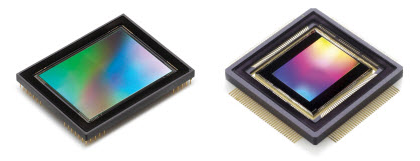
\includegraphics[width=0.5\textwidth]{images/ccd_and_cmos_sensors_210w.png}
		\caption{\label{fig:SensorCCD}{\small Sensor CCD 210W y Sensor CMOS 210W.}}
	\end{figure}
	En general los telescopios (tanto los terrestres como los situados fuera de la atmósfera) constan de una o varias ruedas de filtros (en la figura \ref{fig:irfiltwheel_Hubble} situada en la página \pageref{fig:irfiltwheel_Hubble}, podemos observar una rueda de filtro de rango infrarrojo perteneciente al telescopio espacial Hubble).
	\begin{enumerate}
		\item El color en las imágenes astronómicas:\\
			La información de imagen que almacenan los ficheros FITS carece de información de color, ya que el valor contenido en cada celda que contiene la imagen, se corresponde con la cuenta de fotones que impactan en un determinado tiempo de exposición a una determinada longitud de onda. 
			\\Las imágenes en color que generan las instituciones son el producto de varias (en general 3 o más imágenes en escala de grises). El proceso consiste en asignar un tono a cada imagen y mezclar el resultado en una única imagen. Cada imagen ha sido capturada anteponiendo al detector un filtro físico que deja pasar determinadas longitudes de onda.
			\begin{figure}
				\centering
				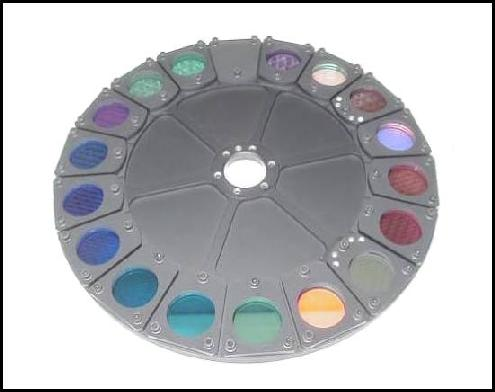
\includegraphics[width=0.25\textwidth]{images/irfiltwheel_Hubble.jpg}
				\caption{\label{fig:irfiltwheel_Hubble}{\small Sensor Rueda Filtros infrarrojos perteneciente al telescopio Hubble.}}
			\end{figure}
			\begin{figure}
				\centering
				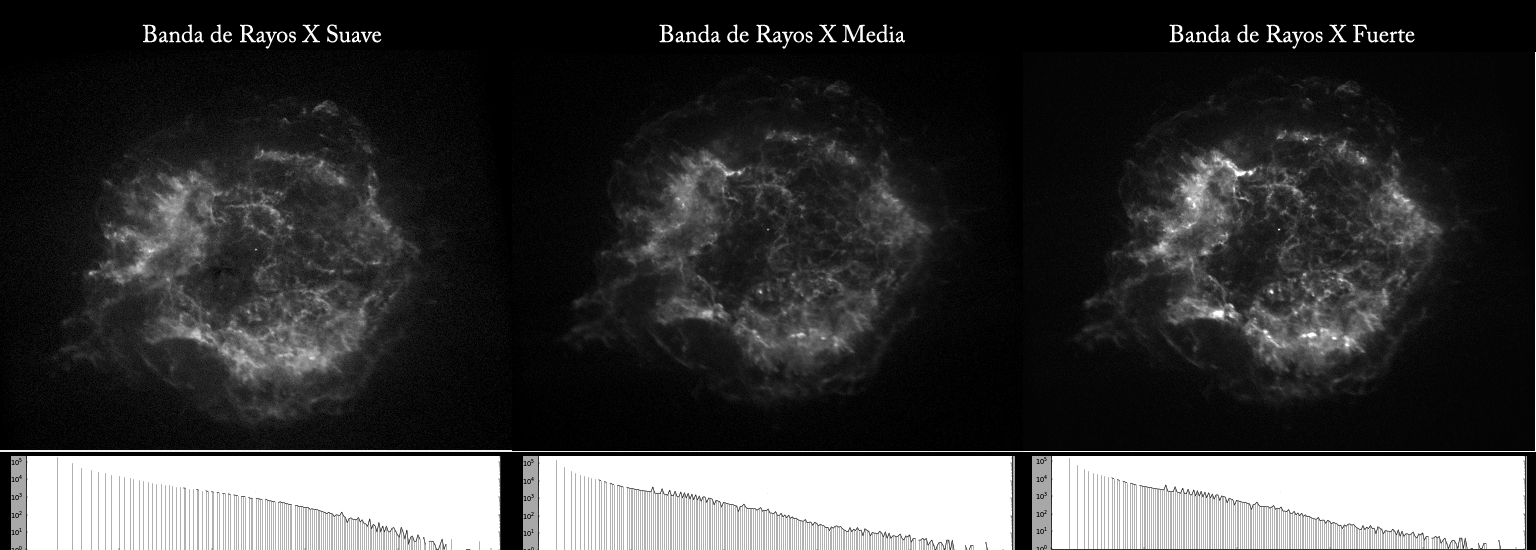
\includegraphics[width=0.5\textwidth]{images/Chandra-Compo-Images.jpg}
				\caption{\label{fig:Chandra Space Telescope Images}{\small Imagenes procedentes de Chandra usando diferentes filtros sobre un mismo apuntado}}
			\end{figure}
			\begin{figure}
				\centering
				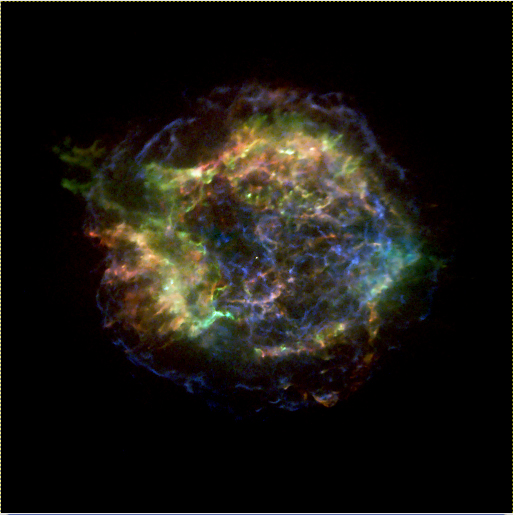
\includegraphics[width=0.25\textwidth]{images/Chandra-Composed-Images.jpg}
				\caption{\label{fig:Chandra_Composed_Images}{\small Composición de imagen en color usando trés imágenes de intensidades, cada imagen se asocia a un canal del espectro RGB}}
			\end{figure}
		\item Detectores profesionales:\\
		El motivo por el cual las imágenes de instrumentos astronómicos profesionales carecen de color, no es otro que el color - o rango visible - aporta muy poca información al ámbito de la astronomía. Es mucho más preciso y aporta más información, obtener un conteo del impacto de fotones en una determinada longitud de onda que una imagen en el espectro visible.
		\\
		Otra de las ventajas es que se simplifica la creación de elementos de detección de imagen. Un detector que captura una imagen en rango visible RGB necesita de tres sensores por cada celdilla, lo que incrementa su coste y reduce su fidelidad al tener que colocar tres dispositivos de captura por cada celda. Esto hace que  inevitablemente desviaciones en la localización exacta de los apuntados o puntos luminosos.
		\\
		En contra nos encontramos con imágenes que carecen del alto impacto visual de las que gozan las imágenes en color.
	\end{enumerate}
	

	\subsection{Imágenes astronómicas amateur}
	Fuera del ámbito académico o técnico, lo habitual es obtener imágenes astronómicas en formatos de imagen genérico tales como TIFF, PNG , o JPG, siendo este último el menos adecuado (el algoritmo de compresión Jpeg destruirá valiosa información \cite{PajaresCruzUCM} de luminancia tal y como  se aprecia en la figura \ref{fig:destroyJPG}).
	\begin{figure}[!htb]
		\centering
		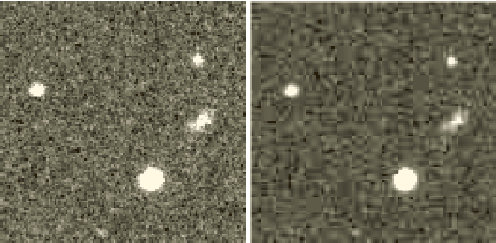
\includegraphics[width=1\textwidth]{images/FITScomprimidoJPG.png}
		\caption{\label{fig:destroyJPG}{\small Efecto de la compresión jpg, a la izquierda la imagen original, a la derecha la imagen comprimida.}}
	\end{figure}
	\begin{figure}[!h]
		\centering
		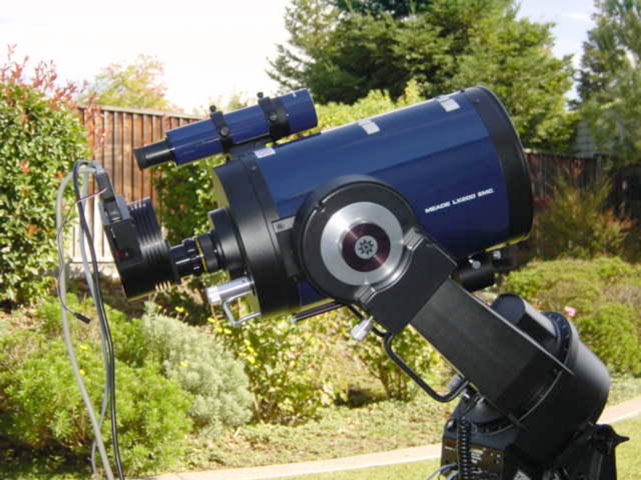
\includegraphics[width=0.65\textwidth]{images/amateur_transit_detection_Schmidt_Cassegrain_765_510pixCCD.jpg}
		\caption{\label{fig:Amateur Telescope}{\small Telescopio amateur de detección de tránsitos Schmidt-Cassegrain de 8 pulgadas, consta de un CCD de 765x510 pixels}}
	\end{figure}
	Estos formatos carecen de información astronómica en sus metadatos y lo más importante, su profundidad de color está generalmente limitada entre 8 bits (paletas indexadas con 256 posibles valores) y 32 bits (8 bits por canal), dividiéndose entre los tres colores base (RGB); con lo que se obtiene (en los casos de 24 y 32 bits) $ 2^8 $ intensidades diferentes, muy lejos de los rangos que manejaremos en el formato FITS.
	\\
	Estas imágenes son capturadas usando tecnología de consumo general, en la mayoría de los casos sensores CCD RGB.
	\\
	\clearpage

 

	\section{Objetivos}
	\label{sec:objetivos}
	En este trabajo se busca explorar nuevos métodos de análisis de imágenes astronómicas, creación de nuevos algoritmos de obtención de elementos de interés o adaptación de los ya existentes.\\
	%Acortar frases, separar.
	Además de los algoritmos se ha desarrollado una interfaz de fácil manejo en la que se muestre tanto el resultado final como parte del proceso intermedio que se realiza, pudiendo variar los parámetros de configuración de los algoritmos y por lo tanto el resultado final.\\
	\\
	El desarrollo se ha planteado de tal forma que está abierto a nuevas funcionalidades, se ha prestado especial atención en que el trabajo realizado, sirva de base futuros algoritmo de aprendizaje automático o machine-learning.
	
	\subsection{Objetivos Generales}
	
	El objetivo principal es la creación de algoritmos que, dada una imagen que representa una sección del espacio exterior, determinen la existencia de estrellas y galaxias.
	\\
	Tras determinar la lista de puntos de interés en la imagen, el software catalogará los objetos mediante la exploración de las vecindades de los puntos destacados y haciendo uso de los algoritmos de visión por computador y criterios estadísticos.
	
	\subsection{Objetivos Específicos}
	Llevar a cabo todo el proceso implica una serie de pasos los cuales se describen a continuación:
	%description mejor
	\begin{itemize}
		\item \textbf{Lectura de imágenes genéricas:}\\
		Implica la lectura de formatos genéricos de imágenes raster y en caso de poseer información de color (multidimensional), trasformar esta información a un espacio de color unidimensional.
		\begin{center}
%%Ampliar
		{\large $G:\mathfrak{\;R^{2}\rightarrow\mathfrak{K^{2}}}$}
		\end{center}
		Siendo G la transformación de un espacio de dimensión 2 del cuerpo $\mathfrak{\;R}$ a un espacio de dimensión 2 del cuerpo de los enteros $\mathfrak{\;K}$ acotado {[}0, $2^{8})$.
		
		\item \textbf{Lectura y calibración automática de imágenes en formato FITS:}\\
		El software ha de ser capaz de transformar el contenido de imagen del fichero FITS a un array de numPy \\
		Tras la lectura se procede al proceso de calibración de la imagen así como una transformación del espacio de color:

		\begin{center}
		{\large 	$F:\mathfrak{\;\mathfrak{R^{2}}\rightarrow\mathfrak{\mathfrak{R'}^{2}}}$}
		\end{center}
		La función $F$ se encargará de descartar los valores menores que cero (posibles errores en el detector o guardado del fichero) en $\mathfrak{R^{2}}$.\\
		En nuestro caso $\mathfrak{R^{2}}$ contiene valores no acotados, cuyo máximo y granularidad dependen del instrumento con el que fue capturada la imagen.\\
		$\mathfrak{R'}^{2}$ almacenará la calibración de la imagen en base a la equalización elegida, bien automáticamente o bien por el usuario.

		
		\item \textbf{Detección de zonas que representen gases o polvo:}\\
		Las estrellas por su naturaleza, iluminan sus proximidades, permitiendo	ver el polvo o gas que las rodea; cuando un cúmulo de estrellas tienen en sus proximidades polvo o gases en suspensión, éstos se ven iluminados. A estas zonas difusas de las imágenes las denominaremos \textbf{halos}.
		\\
		El halo galáctico es un componente extendido, más o menos esférico que se extiende en las proximidades de una galaxia (para más información ver \cite{NASADISKHALO}).
		\\
		La distinción entre el halo y el cuerpo de la galaxia queda claramente definido en las galaxias espirales (ver figura \ref{fig:ESA_GALAXY_Espiral}), donde la forma esférica del halo contrasta con el disco plano o \texttt {flat-disc}. En las galaxias elípticas esta distinción no es clara(ver figura \ref{fig:ESO_GALAXY_Eliptica}), ya que no hay una transición marcada entre el cuerpo de la galaxia y el halo.
		\begin{figure}[!hp]
			\centering
			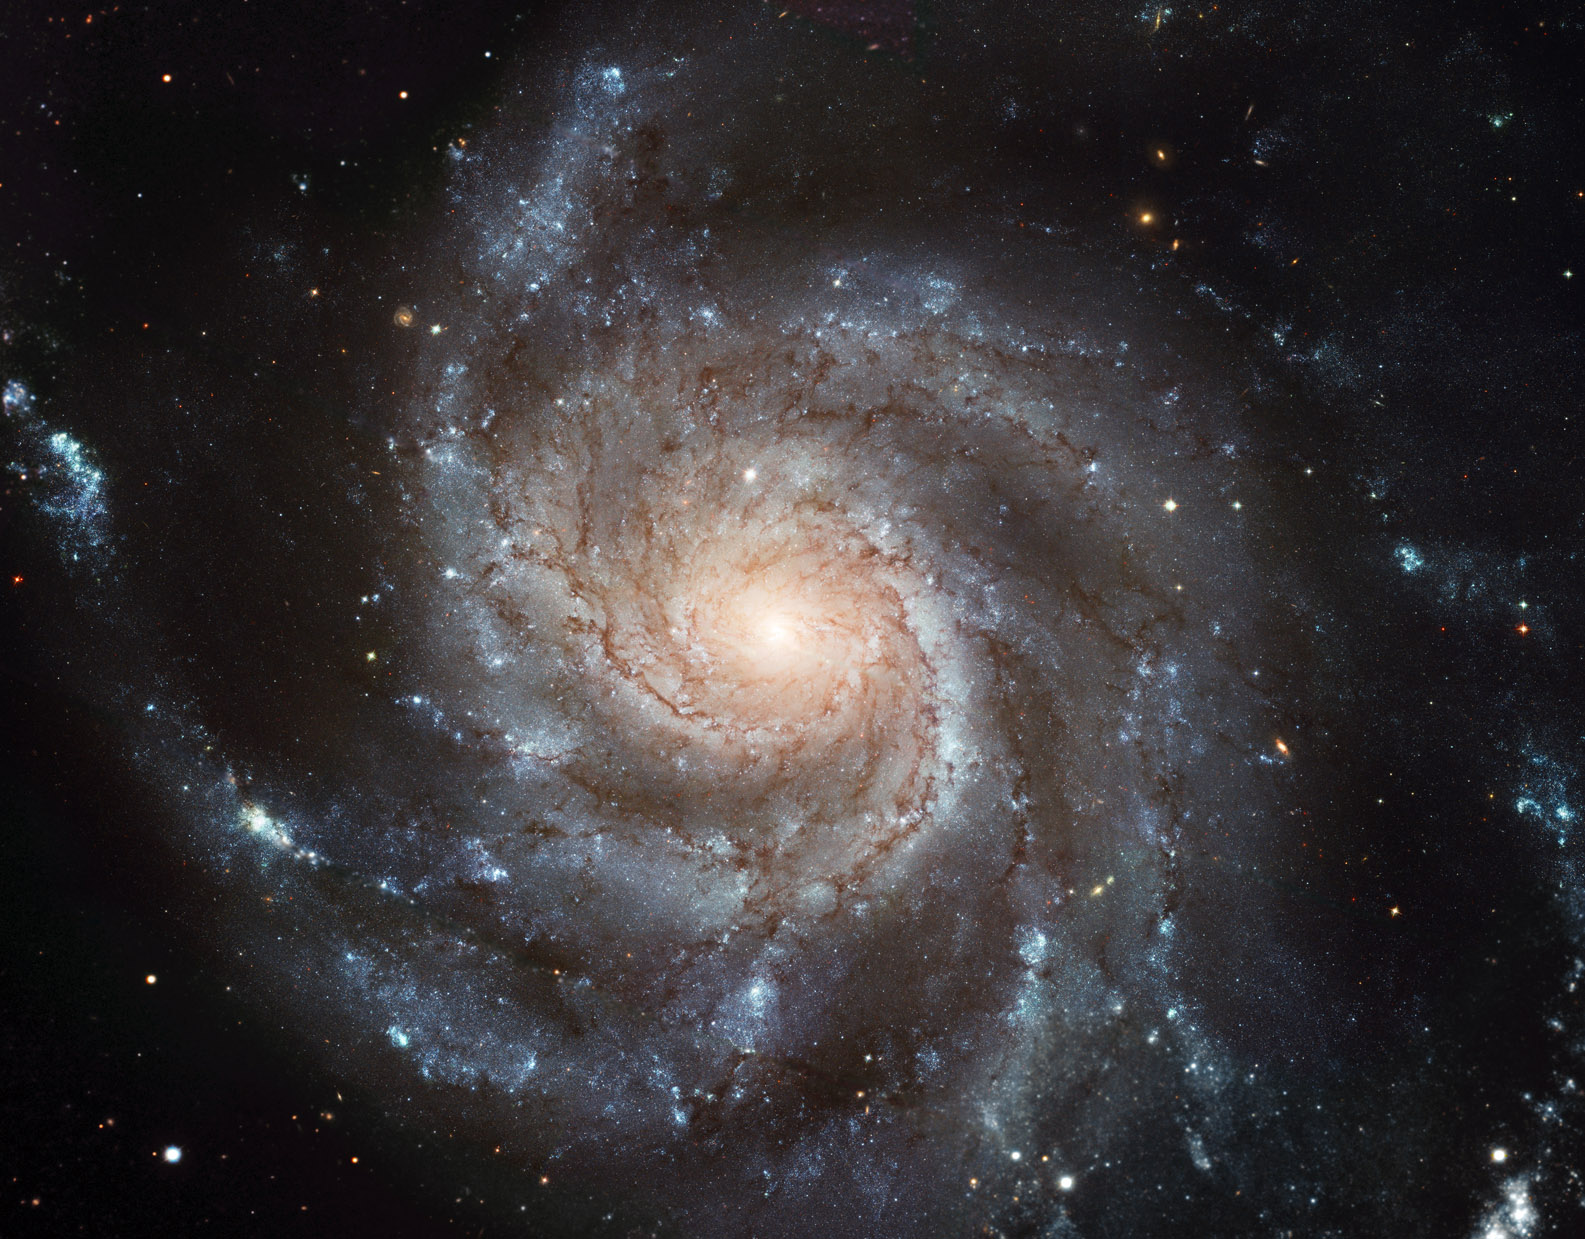
\includegraphics[width=0.3\textwidth]{images/Messier100_NGC5457Galaxy.jpg}
			\caption{\label{fig:ESA_GALAXY_Espiral}{\small Galaxia espiral NGC5457 con halo. Imagen cortesía de la E.S.A.}}
		\end{figure}

		\begin{figure}[!hb]
			\centering
			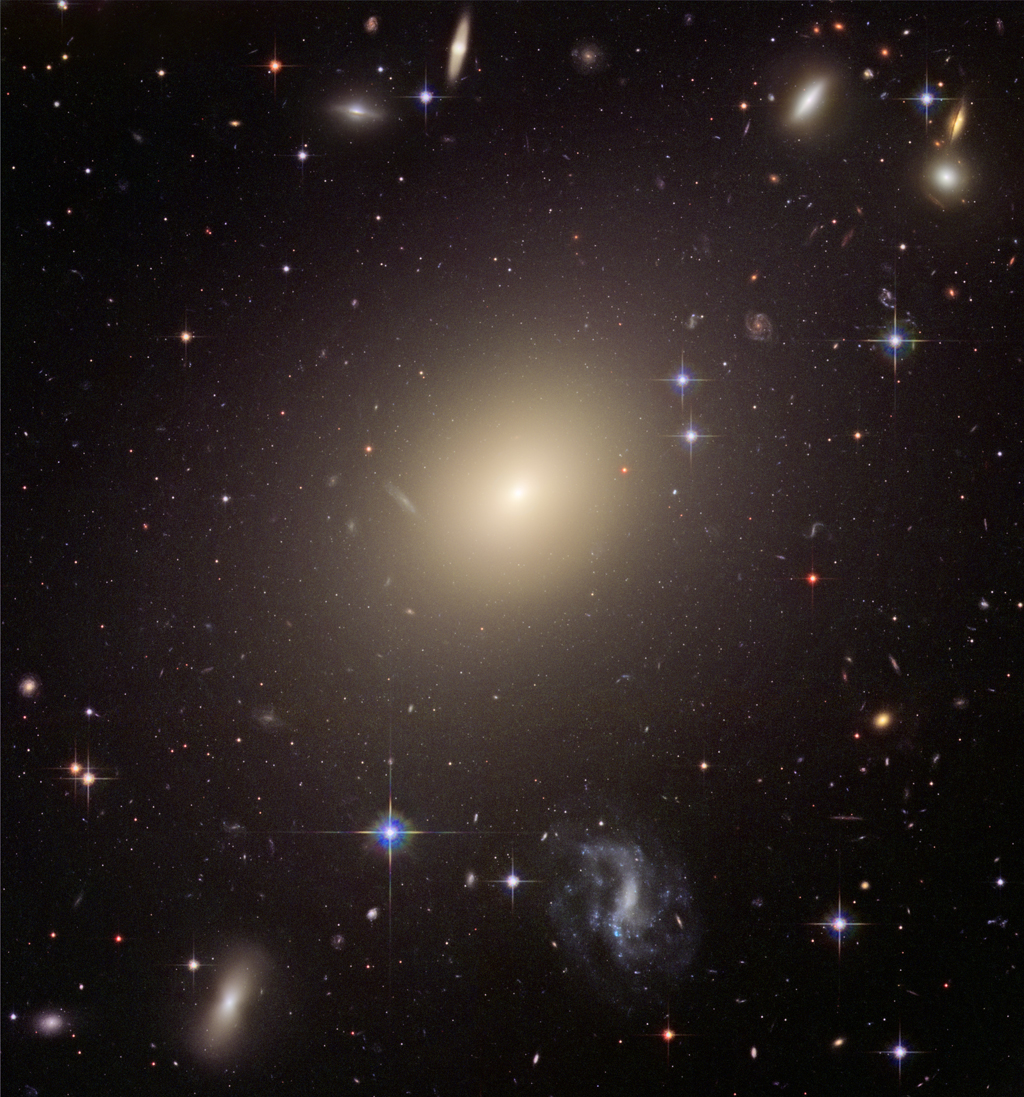
\includegraphics[width=0.28\textwidth]{images/ElipticalGalaxyESO325-G004.jpg}
			\caption{\label{fig:ESO_GALAXY_Eliptica}{\small Galaxia elíptica ESO 325-G004 (en el centro) con halo. Imagen cortesía de NASA/ESA} }
		\end{figure}

		Una característica que usarán nuestros algoritmos, es analizar el gradiente local de los halos alrededor de los puntos de máxima intensidad (ver figura \ref{fig:gradiente}) para determinar la existencia de galaxias.
		
			\begin{figure}[!h]
				\centering
				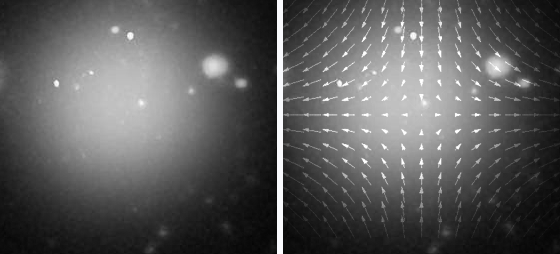
\includegraphics[width=0.4\textwidth]{images/gradiente_GalaxyClusterCLj10001+0220.png}
				\caption{\label{fig:gradiente}{\small Cluster de Galaxias CL J1001+0220, a la derecha detalle del gradiente. Imagen cortesía de NASA/CXC/CEA/T}}
			\end{figure}		


		%ok
		\item \textbf{Eliminación de la función de dispersión de punto (PSF):}\\
		La función de dispersión de punto es un fenómeno que provoca que, dado un punto lumínico y un receptor electrónico, se den dispersiones de los fotones a celdas adyacentes del detector (ver figura \ref{fig:PSF}). 
			\begin{figure}[!h]
				\centering
				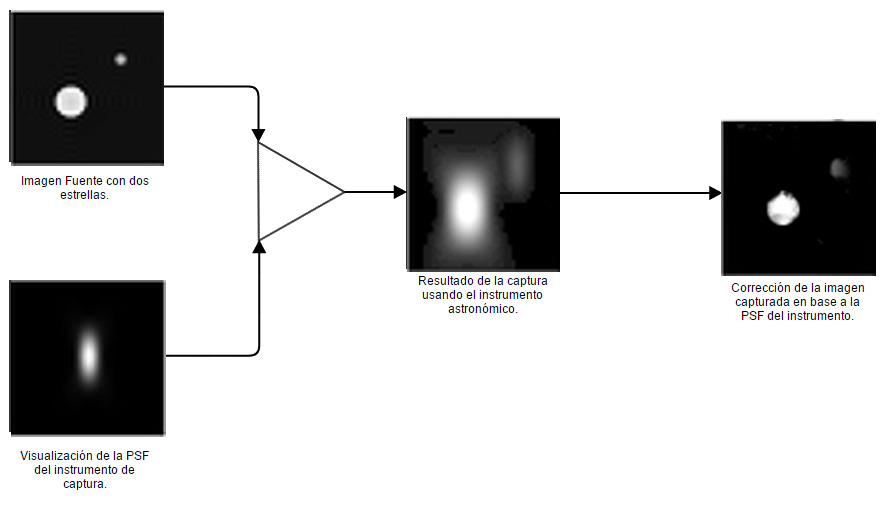
\includegraphics[width=0.9\textwidth]{images/PSF-explicada2.jpg}
				\caption{\label{fig:PSF}{\small Corrección de PSF o función de dispersión de punto}}
			\end{figure}
		\\Un buen detector tendrá una menor PSF que un mal detector.\\
		Eliminando la función de dispersión del punto obtendremos unos resultados que se aproximen más a la realidad.\\

		\item \textbf{Detección del espacio vacío:}\\
		Para un correcto tratamiento de la imagen y facilitar la detección de elementos de interés mediante técnicas de suavizado y análisis por sectores, se determina un rango de color y nivel de ruido que posteriormente se eliminará de la imagen.
		
		\item \textbf{Detección de estrellas puntuales y galaxias:}\\
		Las galaxias son aglomeraciones de estrellas, cuerpos celestes y materia cósmica localizadas en una zona del espacio por efecto de la fuerza de la gravedad y que tienen un movimiento por el espacio en conjunto.\\
		En las inmediaciones de cada estrella perteneciente a una galaxia, es habitual encontrar polvo o gas atrapado por las fuerzas de gravitación existentes (ver figuras \ref{fig:ESO_GALAXY_Eliptica} y \ref{fig:gradiente}).\\

		Las estrellas que no pertenecen a una galaxia se denominan Stellar Outcast\cite{stellarOutcast} ó Intergalactic Stars que al no pertenecer a una galaxia no son capaces de atraer individualmente polvo o nubes de gas.\\
		Aprovechando el gradiente generado por las nubes de polvo y gas, el	algoritmo se encarga de distinguir entre estrellas y galaxias.
		\begin{figure}[!htb]%meter de donde proviene.
			\centering
			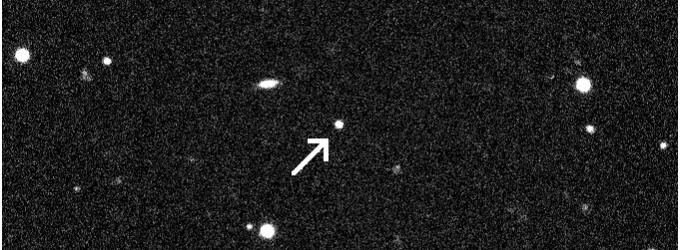
\includegraphics[width=0.4\textwidth]{images/star.jpg}
			\caption{\label{fig:IntergalacticStar}{\small Stellar Outcast SDSS J090745.0+24507}}
		\end{figure}

	\end{itemize}	

	\vfill

	\section{Análisis del problema y plan de trabajo}

	\subsection{Antecedentes }
	
	El único proyecto que hemos encontrado de similares características	es el proyecto Galaxy Zoo. \\
	Galaxy Zoo(https://www.galaxyzoo.org/) comenzó su andadura en 2007. Es un proyecto online de astronomía que invita a sus miembros a ayudar a clasificar alrededor de un millón de galaxias. Es un ejemplo de ciencia ciudadana ya que utiliza la ayuda de gente anónima para ayudar a la investigación científica. \\
	Gran parte del software astronómico hace uso de meta-datos para localizar y dar una clasificación de estrellas y galaxias en función a una base de datos. \\
	Nuestro objetivo es \textit{evitar la dependencia de la interacción humana o el uso de bases de datos}, supliéndola con técnicas de visión artificial.\\

	%
	\subsection{Dificultades identificadas}
	Las peculiaridades de las imágenes astronómicas hacen que los algoritmos existentes en las librerías clásicas de visión por computador no se adapten a lo esperado, esto hace que las imágenes tengan que ser transformadas. Esta transformación no es trivial y cada caso puede presentar peculiaridades.
	\newline
	\\
	Destacamos entre otras, las siguientes dificultades:
	\begin{enumerate}
	%Describir en detalle
	\item \textbf{Calibración de la imagen:}\\
	La calibración de las imágenes FITS a un rango dinámico correcto sobre el cual las librerías de visión artificial puedan operar.
	\item \textbf{Baja resolución de los puntos de interés:}\\
	Los objetos de interés no tienen por qué estar centrados en la imagen, en muchos casos ocupan regiones inferiores a 16x16 pixels. 
	\item \textbf{Ausencia de algoritmos avanzados en la detección de objetos celestes sobre imágenes raster:}\\
	Los algoritmos de catalogación hacen uso de las coordenadas astronómicas presentes en la cabecera del fichero FITS para cruzar estas coordenadas con bases de datos en las que están determinados los astros de interés; nuestro objetivo no es posicionar objetos de interés en base a los datos almacenados en una base de datos sino descubrir posibles objetos de interés en una imagen.
	\item \textbf{Dificultad para conseguir ficheros de prueba:} \\
	Las bases de datos astronómicas existentes contienen grandes cantidades de imágenes cuya forma de acceso se realiza mediante sus coordenadas astronómicas; dando como resultado de la búsqueda una larga lista de imágenes FITS.\\Además el peso de las mismas hace difícil su gestión.
	\end{enumerate}
	\newpage

	\subsection{Diseño de la interfáz de usuario}
	Queremos crear una interfaz de trabajo, la interfáz gráfica ha de tener un doble propósito:
	\begin{enumerate}
		\item Facilitar la configuración de los algoritmos y visualizar el histograma resultante para la correcta automatización.\\ En un futuro trabajo se pretende hacer uso de técnicas de aprendizaje automático. La interfaz serviría como punto de inicio para obtener los parámetros base necesarios para el aprendizaje automático.
		\item Permitir al usuario no especializado trabajar con sus imágenes y obtener el resultado de forma visual.
	\end{enumerate}
	Sería deseable que la interfaz visual sea agradable en apariencia y de fácil manejo, mostrando  las opciones de manipulación que necesita el usuario y los datos más significativos para  nuestros algoritmos.\\
	Se valoraron diferentes tecnologías (QT en sus variante PyQT y PySide), optando por Tkinter por su versatilidad.\\
	Para aprovechar lo mejor posible el area de ventana se habilitará una zona con pestañas en la que se mostrará la imagen original y procesada (para más detalle ver subsección \ref{GUI}).
	
	\subsection{Prueba de los algoritmos}
	Para determinar la validez de los algoritmos, sería deseable disponer de imágenes que incluyen tanto imágenes FITS como imágenes genéricas.\\
	Se partirá de una pequeña batería de imágenes, sobre la cual se aplicarán los algoritmos que se desarrollarán (para más detalle ver sección \ref{ownLib}), de este modo podremos afinar su precisión.
	Esta fase ha permitido realizar la automatización del proceso afinando los algoritmos de clasificación.
	Las imágenes usadas como batería de test han sido:
	\begin{enumerate}
		\item \textbf{m10.fits:} cúmulo globular NGC 6254.
		\item \textbf{218wmos.fits:} Imagen ultravioleta tomada de NASA/ESA Hubble Space Telescope WFPC2.
		\item \textbf{casa0.5-1.5keV.fits y casa1.5-3.0keV.fits:} imágenes de Cassiopeia A (Cas A). Muestra un remanente de supernova. La imagen proviene del Hubble Legacy Archive (https://hla.stsci.edu/).
		\item \textbf{blue.fits y red.fits:} imágenes de NGC4038 o galaxia Antennae de la constelación de Corvus, obtenidas mediante dos filtros (rojo y verde). Ambas imágenes fueron tomadas del proyecto NAO-IRAF.
		\item \textbf{Gravitational lensing in the galaxy cluster Abell 370.jpg:} cúmulo de galaxias Abell 1689, presenta una lente gravitatoria. Fuente de la imagen: Hubble Space Telescope (https://www.spacetelescope.org/images/heic0910b/).
		\item \textbf{noReal.jpg:} imagen de simulación de galaxia espiral.
		\item \textbf{image 3417 1e-LEDA-1852.jpg:} Galaxia espiral MCG+01-02-015 Fuente: ESA/Hubble, NASA and N. Gorin (STScI). \\http://www.spacetelescope.org/images/potw1545a/
		\item \textbf{o-HUBBLE-UV-900.jpg:} Imagen compuesta por multiples frecuencias (del ultravioleta al infrarojo), Fuente: Hubble Ultra Deep Field.\\ http://apod.nasa.gov/apod/ap140605.html
		\item \textbf{spiral-galaxy-eso-137-hubble.jpg:} Galaxia espiral ESO 137-001 del Supercúmulo de Virgo, aparece en la parte superior izquierda la anomalía conocida como \textit{El gran atractor}. Fuente: E.S.A.\\Z
		http://sci.esa.int/hubble/53751-spiral-galaxy-spills-blood-and-guts-heic1404/
		\item \textbf{potw1143a.jpg:} Galaxia de estrellas enanas en la constelación del Phoenix.\\
		Fuente:  ESA/Hubble y NASA. (https://www.spacetelescope.org/images/potw1143a/)
		\item \textbf{hubble-galaxy 1743872i.jpg:} Galaxia en la constelación del Agula (IRAS 19399-1026).\\ Imagen simulada.
		Fuente: E.S.A. NASA.\\ http://www.nasa.gov/sites/default/files/thumbnails/image/hubble\char`_friday\char`_05062016.jpg
	\end{enumerate}
	Se han tenido en cuenta tanto imágenes FITS (4 imágenes con dos variantes de filtros)como imágenes raster (7 imágenes) de contenido astronómico (una de ellas es simulada).\\

	\begin{figure}[!htb]
		\centering
		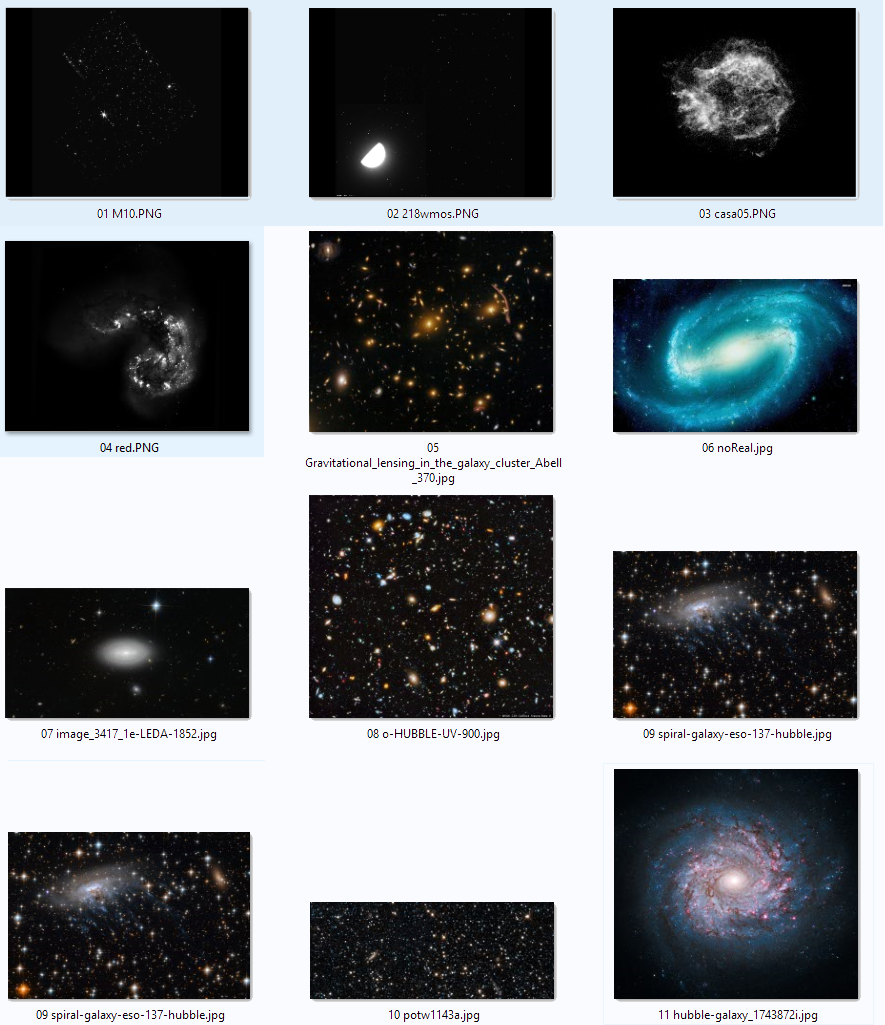
\includegraphics[width=1.2\textwidth]{images/imgFuentesSnap/compoFuentes.png}
		\caption{\label{fig:IntergalacticStar}{\small Muestra de imágenes usadas.}}
	\end{figure}
	\clearpage

	\section{Desarrollo}
	\subsection{Arquitectura interna}
	Todo el desarrollo se ha centrado en el uso del lenguaje Python: es un lenguaje maduro con una gran cantidad de bibliotecas de apoyo. Tanto las bibliotecas usadas como el interprete de Python son de código abierto.\\
	La aplicación se divide en dos ficheros:
	\begin{itemize}
	\item ide.py: contiene la creación de la interfaz gráfica, el flujo que sigue el tratamiento de cada imagen y la parte encargada de la automatización.\\ Se ha usado un enfoque orientado a objetos.
	\item cvSpace.py: en este fichero se encuentran las funciones encargadas del análisis y tratamiento de las imágenes, funciones que hemos dividido en dos grupos: el grupo de la parte estadística y el grupo del tratamiento de imágenes.\\ Este fichero usa un enfoque imperativo.
	\end{itemize}
	
	 Hacemos especial hincapié en el uso de código abierto, ya que dentro de los objetivos del proyecto está la creación de un conjunto de herramientas que puedan ser usadas, modificadas y copiadas libremente por la comunidad; por ello, todo el código se ha desarrollado bajo la licencia BSD.
	\subsection{Bibliotecas externas}
	\paragraph{OpenCV}
	Es una librería de visión artificial, desarrollada bajo la licencia BSD y creada inicialmente por Intel. Es multiplataforma con su núcleo en C y tiene envolturas para gran cantidad de lenguajes, entre ellos Python. Es la librería más avanzada que existe para visión artificial, destacando por su optimización que permite la realización de aplicaciones en tiempo real. OpenCV es una librería madura (se inicio en 1.999) sobre la que gran cantidad de proyectos se apoyan.\\
	\paragraph{NumPy}
	Numpy es el paquete base fundamental para cálculos científicos en el entorno de Python. Al usar Numpy podemos expresar las imágenes como matrices multidimensionales. Esta representación de las imágenes en arrays de NumPy no solo es eficiente desde el punto de vista computacional sino también en la gestión de recursos y nos abre la posibilidad de conectar con otras librerías que usan NumPy. Sus puntos fuertes son:
	\begin{itemize}
		\item Capacidad de manejo de matrices de datos genéricos que usaremos para guardar y manipular nuestras imágenes.
		\item Alta velocidad en las operaciones que se realizan sobre las matrices.
		\item Multitud de funciones matemáticas implementadas de serie.
		\item NumPy es la base de otras librerías, como por ejemplo scikit-learning, librería de aprendizaje automático.
	\end{itemize}
	La licencia de NumPy es BSD.
	\paragraph{Matplotlib}
	Librería de dibujo en 2D/3D que destaca por su facilidad de manejo y potencia. Es la encargada de mostrar los histogramas en la interfaz gráfica.\\
	La licencia de Matplotlib es BSD.
	\paragraph{Astropy}
	Astropy es un proyecto comunitario para acercar a python al mundo de la astronomía. Su núcleo está desarrollado en C y Python. El proyecto Astropy busca crear un framework robusto con las funcionalidades generales que se requieren en astronomía. Sus desarrolladores y usuarios principales son profesionales de las astronomía y al ser un proyecto comunitario cubre muchos de sus ámbitos (fotometría, spectrografía, sistemas de coordenadas, etc).\\
	La principal funcionalidad que usamos de Astropy es un módulo que nos permite la carga de ficheros FITS.\\
	La licencia de astropy es BSD.\\
	\paragraph{Tkinter}
	Es la librería de facto ( y más usada ) para desarrollar interfaces gráficas en python. Se basa en TcL/Tk lo que le permite ser multiplataforma y crear interfaces nativas sobre el sistema operativo en el que se esté ejecutando. Toda la interfáz gráfica se apoya en esta librería.\\	
	La licencia de Tkinter es Python License.
	\vfill
	\newpage
	\subsection{Bibliotecas propias}\label{ownLib}
	%Vincular con objetivos
	El desarrollo englobado en esta sección está directamente relacionado con los objetivos propuestos, partiendo de la lectura de imágenes genéricas como de imágenes en formato astronómico FITS, así como los algoritmos que se encargarán del preprocesado necesario para disponer de una imagen transformada que finalmente será procesada por los algoritmos de clasificación.\\
	El resultado de esta secuencia de procesos nos dará una clasificación de los elementos de interés. \\
	Los algoritmos desarrollados los hemos englobado en el fichero cvSpace.py cuyo cometido es realizar todas las tareas de Visión por computador que nos planteamos en los objetivos y estadística; se destacan:
	\paragraph{Ajuste de rango dinámico}
	Su principal cometido es trasladar el rango de intensidades de cada elemento de la matriz imagen a unos rangos normalizados. De especial interés en este \\
	

	\begin{enumerate}
		\item \textbf{Lineal}\\
		Conocidos el máximo $M$ y el mínimo $m$ valor en la matriz, realiza
		la siguiente transformación dando como resultado la figura \ref{fig:HDRLineal}.
			\begin{center}
				{\large $Pixel'[x,y]=\frac{2^{8}*(Pixel[x,y]-m)}{(M-m)}$}				
			\end{center}
			
			\begin{figure}[!htb]
				\centering
				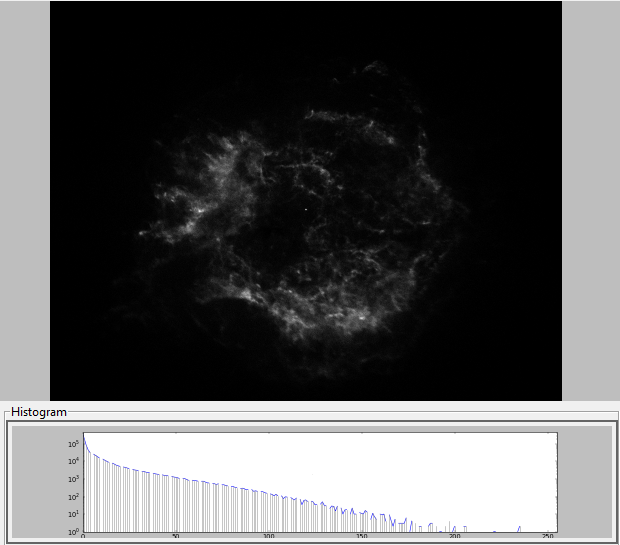
\includegraphics[width=0.4\textwidth]{images/HDREQ/chandraLineal.PNG}
				\caption{\label{fig:HDRLineal}{\small Ajuste de rango dinámico lineal}}
			\end{figure}
		\newpage
		\item \textbf{Raíz cuadrada}\\
		Conocidos el máximo $M$ y el mínimo $m$ valor en la matriz, realiza
		la siguiente transformación (Ver figura \ref{fig:HDRSQRT}):
		El resultado del valor del nuevo pixel se almacena en $Pixel'[x,y]$.
			\begin{center}
			{\large $Pixel'[x,y]=\frac{2^{8}*(Pixel[x,y]-m)}{\sqrt{M-m}}$}			
			\end{center}
			\begin{figure}[!htb]
				\centering
				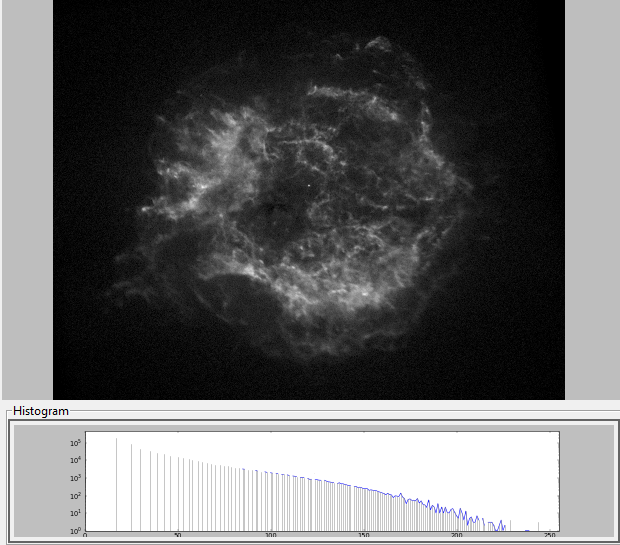
\includegraphics[width=0.5\textwidth]{images/HDREQ/chandraSqrt.PNG}
				\caption{\label{fig:HDRSQRT}{\small Ajuste de rango dinámico Raíz Cuadrada}}
			\end{figure}
		\item \textbf{{}Logaritmo}\\
		Conocidos el máximo $M$ y el mínimo $m$ valor en la matriz, realiza
		la siguiente transformación (Ver figura \ref{fig:HDRLOG}):
			\begin{center}
				{\large $Factor=log_{10}(M-m)$\\
				$Pixel'[x,y]=\frac{log_{10}(Pixel[x,y])}{Factor}$
				}
			\end{center}	
			\begin{figure}[!htb]
				\centering
				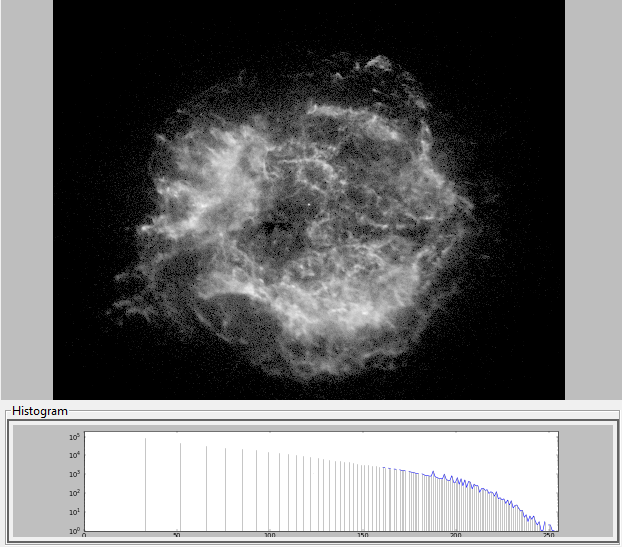
\includegraphics[width=0.5\textwidth]{images/HDREQ/chandraLog.PNG}
				\caption{\label{fig:HDRLOG}{\small Ajuste de rango dinámico logarítmico}}
			\end{figure}

		\item \textbf{Potencia}\\
		Conocidos el máximo $M$ y el mínimo $m$ valor en la matríz y dado
		un exponente n, realiza la siguiente transformación (Ver figura \ref{fig:HDRPOW}):
		\\
		\begin{center}
			{\large $Factor=\frac{1}{(M-n)^{n}}$}
			\\
			{\large $Pixel'[x,y]=(Pixel[x,y]-m)^{n}*Factor$}
		\end{center}
			\begin{figure}[!htb]
				\centering
				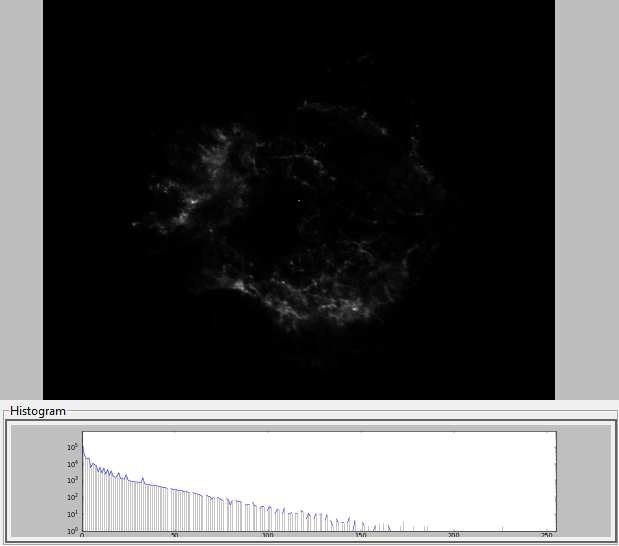
\includegraphics[width=0.5\textwidth]{images/HDREQ/chandraPow1_5.PNG}
				\caption{\label{fig:HDRPOW}{\small Ajuste de rango dinámico potencia con valor 1.5}}
			\end{figure}


		\clearpage
		\item \textbf{Arcoseno Hiperbólico}\\
		Conocidos el máximo $M$ y el mínimo $m$ valor en la matríz y dado
		un factor de no linealidad nL, realiza la siguiente transformación  (Ver figuras \ref{fig:HDRasinh1_5} para nL=1.5 y \ref{fig:HDRasinh5} para nL=5):\\
			\begin{figure}[!htb]
				\centering
				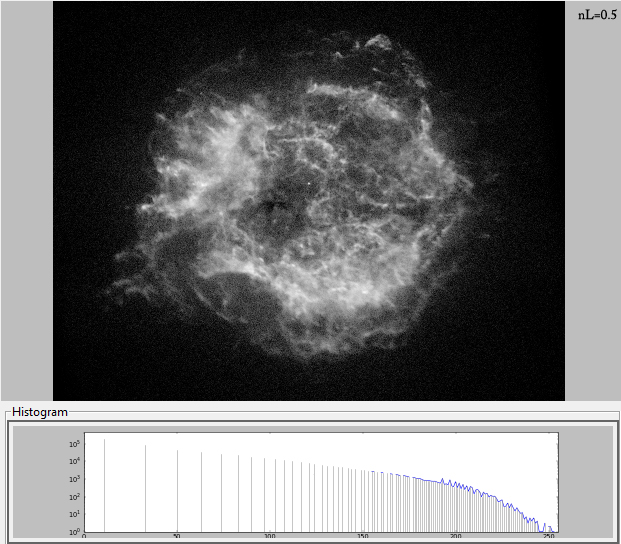
\includegraphics[width=0.4\textwidth]{images/HDREQ/chandraaSinH_0_5.jpg}
				\caption{\label{fig:HDRasinh1_5}{\small Ajuste de rango dinámico ArcoSeno hiperbólico con valor 1.5}}
			\end{figure}
			\begin{figure}[!htb]
				\centering
				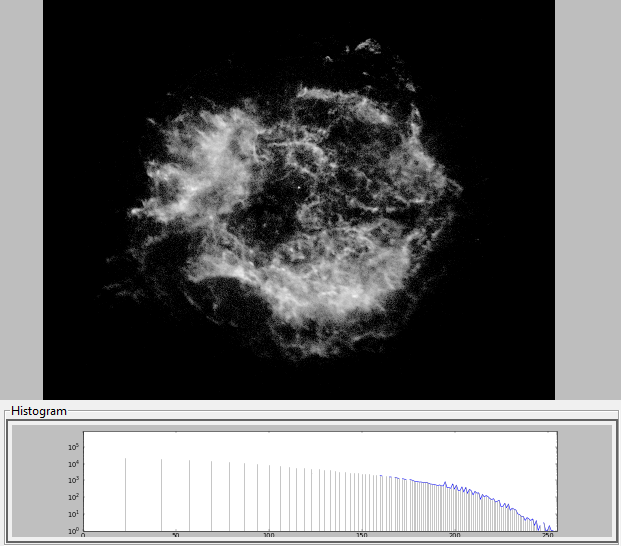
\includegraphics[width=0.4\textwidth]{images/HDREQ/chandraaSinH_5.PNG}
				\caption{\label{fig:HDRasinh5}{\small Ajuste de rango dinámico ArcoSeno hiperbólico con valor 1.5}}
			\end{figure}
			\begin{center}
				{\large $Factor=\frac{arcSinH((M-m)}{nL}$}
				\\
				{\large $Pixel'[x,y]=\frac{\frac{arcSinH(Pixel[x,y]-m)}{nL}}{Factor}$}
			\end{center}
		\vfill


		\item \textbf{Ajuste en base al histograma}\\
			La ecualización del histograma de una imagen es una transformación que pretende obtener un histograma de la imagen con una distribución uniforme. Es decir, que exista el mismo número de pixels para cada nivel de gris del histograma de una imagen monocroma, ocupando todo el rango. (Ver figura \ref{fig:HDRHistograma}).
			\begin{figure}[!htb]
				\centering
				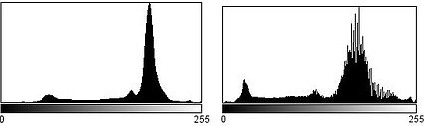
\includegraphics[width=0.4\textwidth]{images/histEqualizado.jpg}
				\caption{\label{fig:HDRHistograma}{\small Ajuste de rango dinámico por ecualización de histograma; a la derecha histograma original, a la izquierda histograma equalizado.}}
			\end{figure}
	\end{enumerate}

	\paragraph{Búsqueda de puntos de interés, estrellas y galaxias}
	%meter referencias, introducir de que es cada puntyo.
	En este punto se detallan las funciones creadas para obtener el objetivo del trabajo, la determinación de objetos de interés.
	\\Varias funciones son las encargadas de buscar, descartar y catalogar las posibles estrellas y galaxias.\\
	Destacamos por su interés \emph{getObjectList}, \emph{getGalaxyCenter} y \emph{getcontours}.\\
	\begin{enumerate}
	\item \textbf{getObjectList}\\
	La función getObjectList presente en cvSpace.py hace uso de la técnica detección de blobs de OpenCV \cite{OpenCV} para localizar puntos de interés, concretamente los \textit{candidatos a estrellas}.\\
	La búsqueda mediante blobs\footnote{Un blob es una región de la imagen que difiere en sus propiedades como color o intensidad, con respecto a sus vecindades} se centra en la variación de la intensidad de cada pixel con su vecindad; el proceso en detalle realiza las siguientes operaciones:
	\begin{enumerate}
		\item Convierte la imagen a una imagen binaria.
		\item Extrae las componentes conectadas en base a un cálculo de contornos.
		\item En caso de blobs muy cercanos entre sí, los agrupa en un único blob. Este proceso  es de especial interés para la agrupación de estrellas que conforman una galaxia.
		\item Se eliminan aquellos blobs que son detectados de forma errónea; para ello se hace uso de la imagen de espacio vacío generada mediante el método {\scriptsize generateDarkImage} de la clase AstroImage.\\
		Se descartan aquellos candidatos cuyo centro de coordenadas ha caído sobre la zona marcada como espacio vacío, conservándose el resto (ver figura \ref{fig:removePointsConparation}).
		\begin{figure}[!htb]
			\centering
			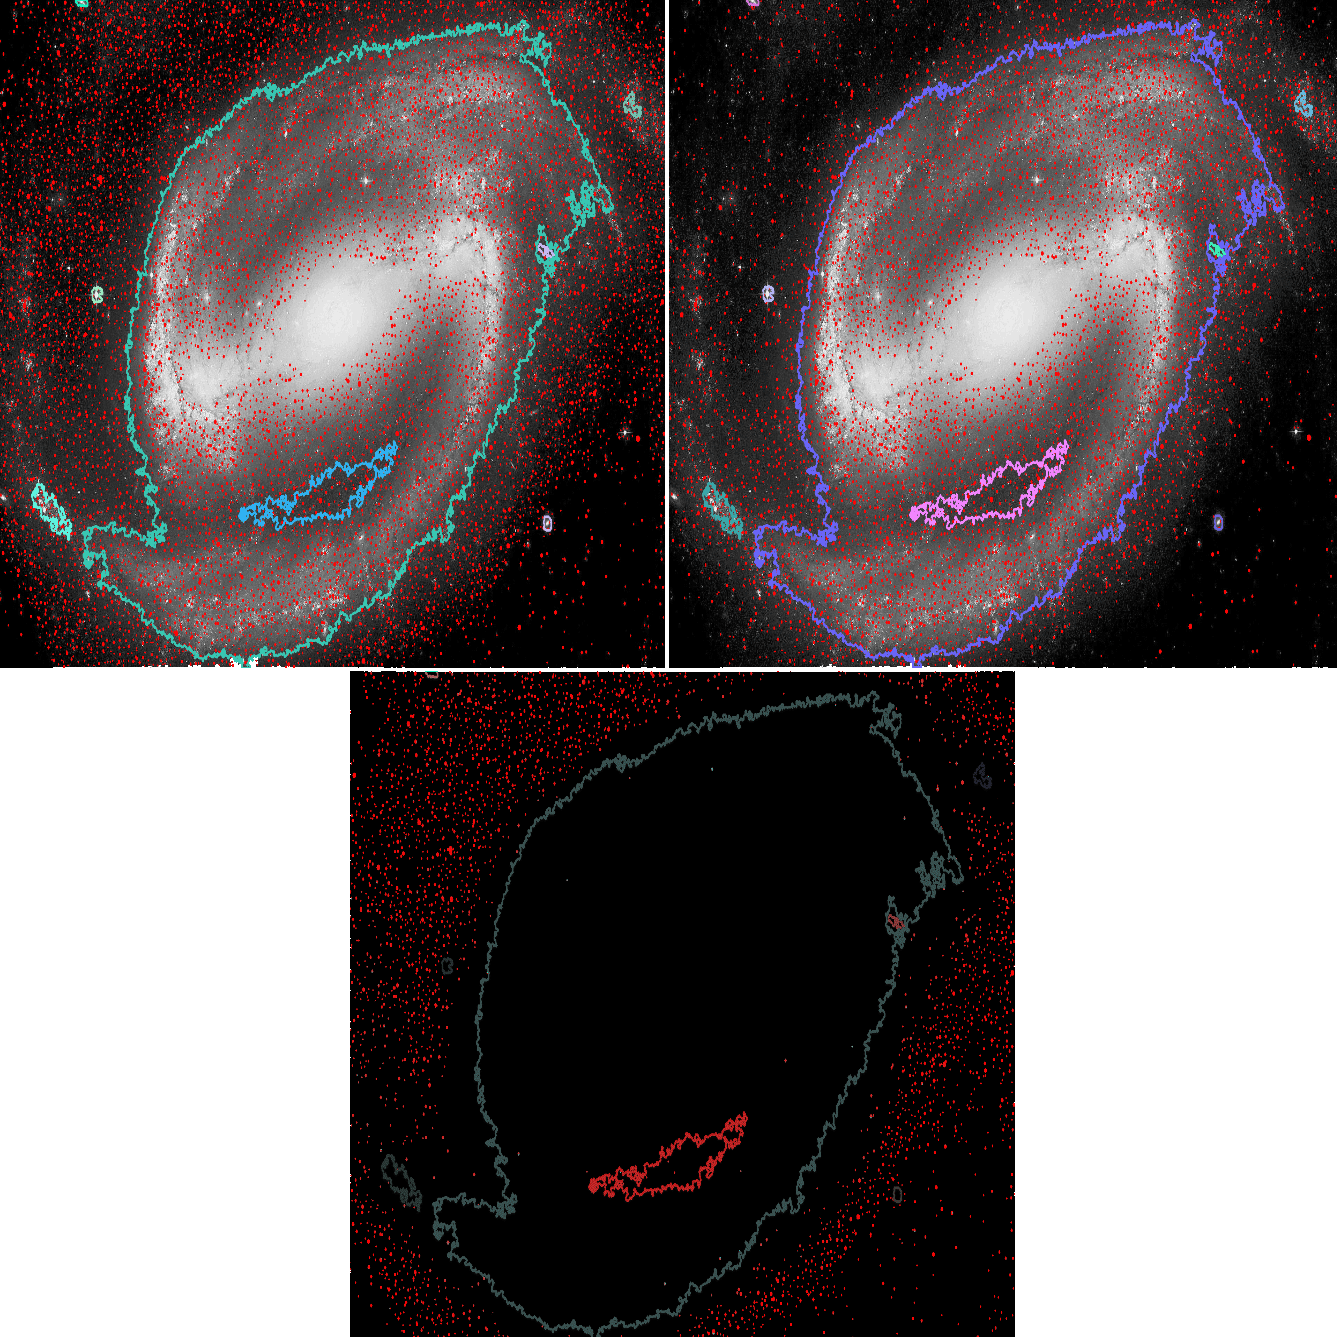
\includegraphics[width=0.9\textwidth]{images/removeBadPoints3.png}
			\caption{\label{fig:removePointsConparation}{\small Resultado del proceso de categorización y eliminación de puntos de interés erróneos.}}
		\end{figure}

		
		\item Para cada grupo de blobs nos devuelve tanto su centro como su área.
	\end{enumerate}
	\item \textbf{getGalaxyCenter}:	\\
	%hacer una macro para los nombres de las funciones
	La función {\scriptsize getGalaxyCenter} se encarga de determinar el centro de las candidatas a galáxias.\\
	El proceso que realiza {\scriptsize getGalaxyCenter}, se resume en los siguientes pasos:
	\begin{enumerate}
		\item Aplicación de blur a la región de interés.
		\item Búsqueda del máximo local en intensidad.
	\end{enumerate}

	Es necesario realizar un blur \footnote{Blur: es una operación simple y frecuente en el procesado de imágenes para eliminar el ruido aplicando un suavizado. El suavizado se consigue  mediante la siguiente transformación: $g(i,j)=\sum_{k,l}f(i+k,j+l)*h(k,l)$ siendo $h(k,l)$ los coeficientes del filtro (también denominados Kernel)} o difuminado, como se aprecia en las imágenes \ref{fig:galaxiCenterFromImage_01_ERROR} \ref{fig:galaxiCenterFromImage_02_Blur} y \ref{fig:galaxiCenterFromImage_03_Correct}.\\
	En caso de no aplicar el suavizado a la imagen, el pico de mayor intensidad no tendría por qué estar situado en el centro de la galaxia. Al aplicar el suavizado, se pondera en media el valor de cada pixel con su vecindad y aumentará la probabilidad de que el centro calculado se ajuste al centro de la galaxia. Esto es debido a que en el centro de la galaxia se acumula la mayor área lumínica.
	\begin{figure}[!htb]
		\centering
		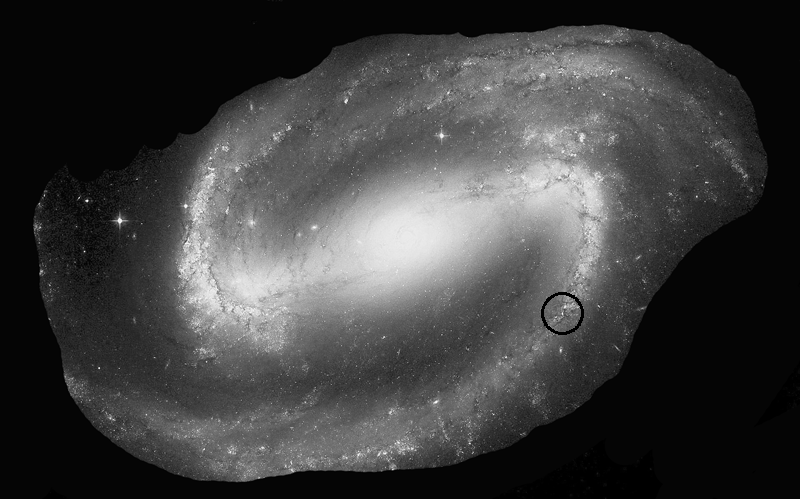
\includegraphics[width=0.5\textwidth]{images/galaxiCenterFromImage_01_ERROR.png}
		\caption{\label{fig:galaxiCenterFromImage_01_ERROR}{\small Obtención errónea del centro de la galaxia (marcado con una circunferencia) al aplicar la función {\scriptsize getGalaxyCenter} sobre la imagen sin procesar con un filtro de suavizado.}}
	\end{figure}
	\begin{figure}[!htb]
		\centering
		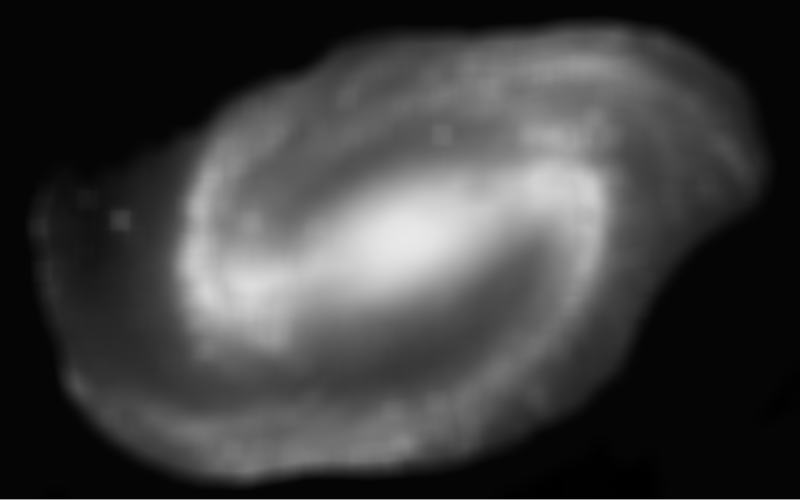
\includegraphics[width=0.5\textwidth]{images/galaxiCenterFromImage_02_Blur.png}
		\caption{\label{fig:galaxiCenterFromImage_02_Blur}La imagen original ha sufrido el proceso de suavizado.}
	\end{figure}
	\begin{figure}[!htb]
		\centering
		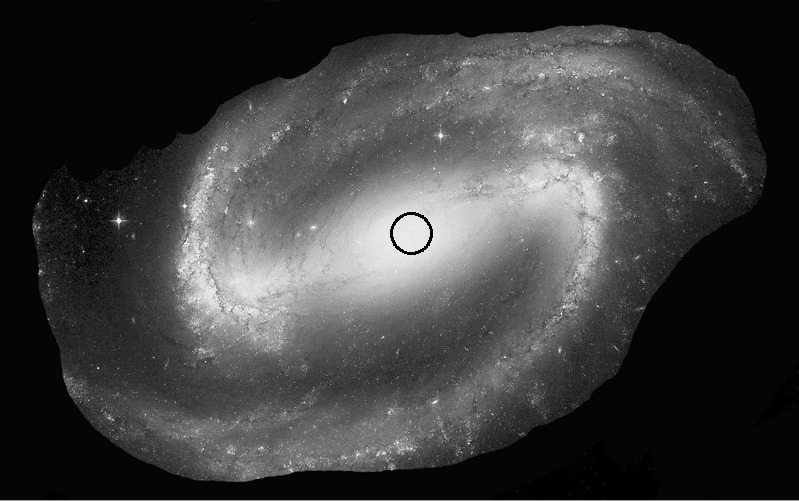
\includegraphics[width=0.5\textwidth]{images/galaxiCenterFromImage_03_Correct.png}
		\caption{\label{fig:galaxiCenterFromImage_03_Correct}{\small Obtención correcta del centro de la galaxia (marcado con una circunferencia) al aplicar la función {\scriptsize getGalaxyCenter} sobre la imagen procesada con un filtro de suavizado.}}
	\end{figure}
	\clearpage
	\item \textbf{getContours}:	\\
	{\scriptsize getContours} aplica búsquedas de contornos sobre la imagen transformada para detectar formaciones de galaxias e internamente realiza operaciones de erosión, dilatación y cierres de contornos.A modo descriptivo del proceso, se presenta el código usado.
	\end{enumerate}
	\lstinputlisting[language=Python, frame= single, columns=fullflexible, firstline=1, lastline=36]{getContoursSimplified.py}

	\paragraph{Eliminación de ruido y Point Spread Function (PSF)}
	\begin{enumerate}
	\item Eliminación de ruido:
	En base al resultado del algoritmo de búsqueda de contornos, se eliminan áreas carentes de interés y producto del ruido.
	\\El algoritmo realiza cálculos incrementales del número de contornos, estimando el ruido por el crecimiento a cada iteración. Si de una iteración a la siguiente el número de contornos crece en un factor de más del doble, se estima que se ha llegado a un umbral correcto.
	\\
	La eliminación del ruido en nuestro caso es una tarea compleja, ya que la diferencia entre una región de ruido y una región que contiene una estrella resulta difícil hasta para un ojo entrenado.
	\newline
	\item Eliminación de PSF:\\
    Aplicando operaciones morfológicas sobre la imágen, concretamente una dilatación seguida de una erosión, se eliminan los puntos detectados erróneamente como válidos.
    \\
    Para la eliminación de la PSF se ha estimado, en base a los test realizados, usar un kernel\footnote{Kernel es una matriz bi-dimensional (normalmente de pequeño tamaño) de coeficientes, que se usa en la convolución de imágenes. } de tamaño 5.
    	\begin{figure}[!htb]
    		\centering
    		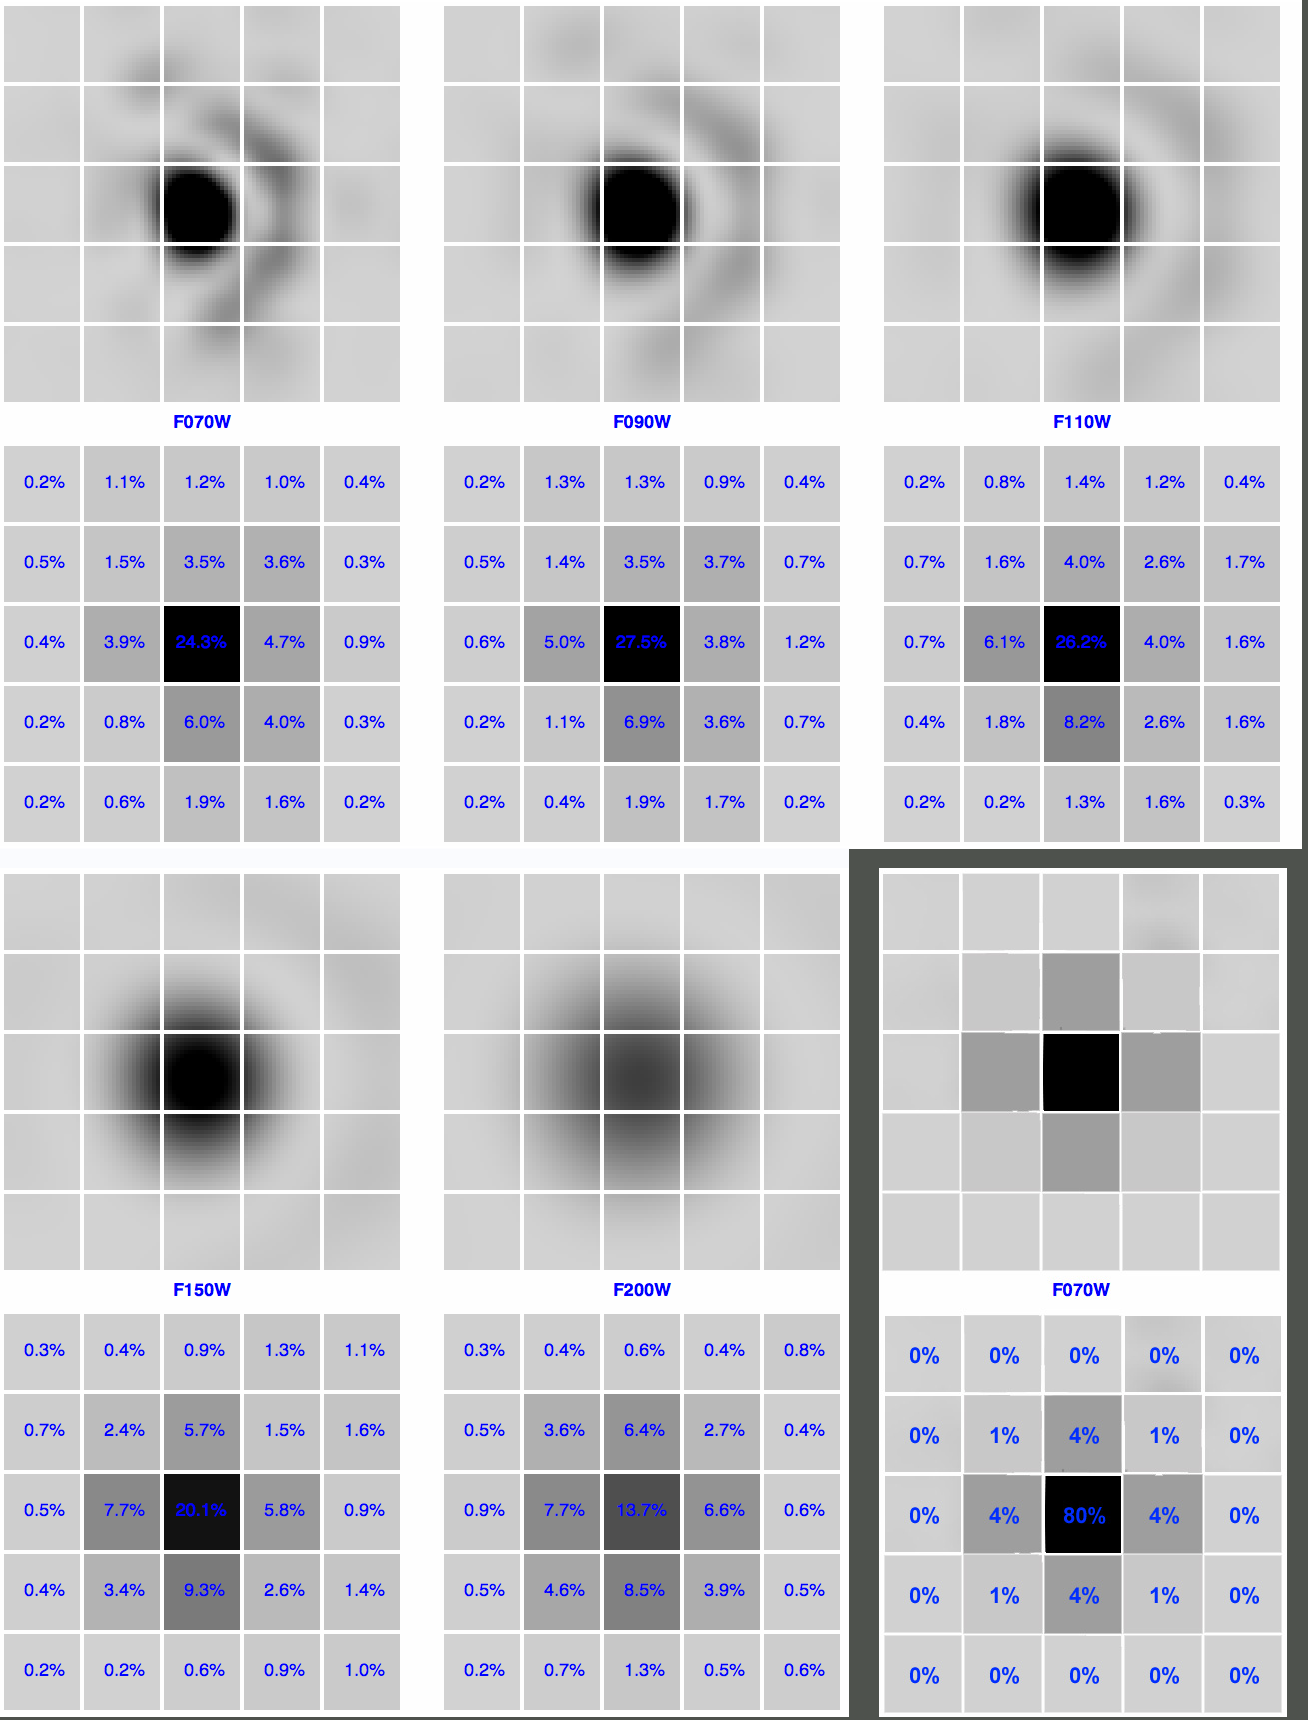
\includegraphics[width=1\textwidth]{images/PSFUnificadas.png}
    		\caption{\label{fig:psfInfrared}{\small Distintas PSF (5) de un instrumento astronómico al aplicar diferentes filtros físicos de longitud de onda. La última imagen (inferior derecha) se corresponde con la simulación de reducción de PSF}}
    	\end{figure}
	Como se aprecia en la figura (\ref{fig:psfInfrared}), la forma que toma la PSF varía según el filtro físico usado al captar la imagen dese el telescópio, presentando formas cercanas a una Normal N-Dimensional.

	\end{enumerate}
	%\subsubsection{Determinación de forma en las galaxias}
	\clearpage
	\subsection{Procesado de imágenes}
	\paragraph{Pre-procesado base}
	El siguiente esquema detalla el proceso que sigue cada imagen y al que llamaremos pre-procesado base. (Ver figura \ref{fig:esquemaPreprocesado})\\
	\begin{figure}[!htb]
		\centering
		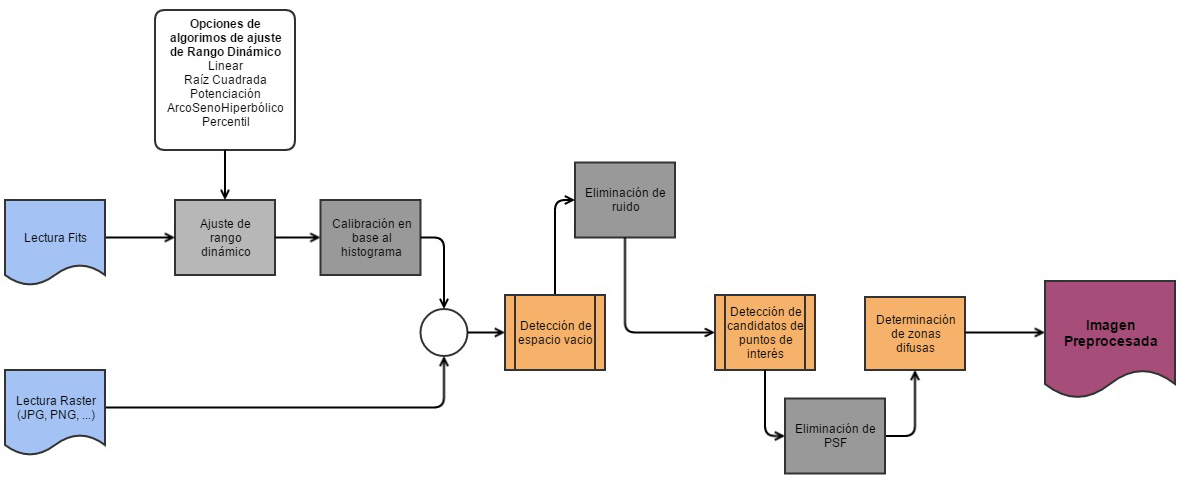
\includegraphics[width=1\textwidth]{images/tfg2016pipeline1.jpg}
		\caption{\label{fig:esquemaPreprocesado}Flujo de pre-procesado}
	\end{figure}
	En el caso de la carga de una imagen astronómica FITS se realiza un ajuste del rango dinámico, este paso se obvia para las imágenes en formato raster genérico ya que se presupone que el instrumento de captura tiene por salida una imagen en el rango esperado.\\ \\
	La imagen FITS se convierte a una matiz de 8 bits, cuyo contenido dependerá de la ecualización aplicada (Ver figura \ref{fig:distintasEqu}).\\
	\begin{figure}[!htb]
		\centering
		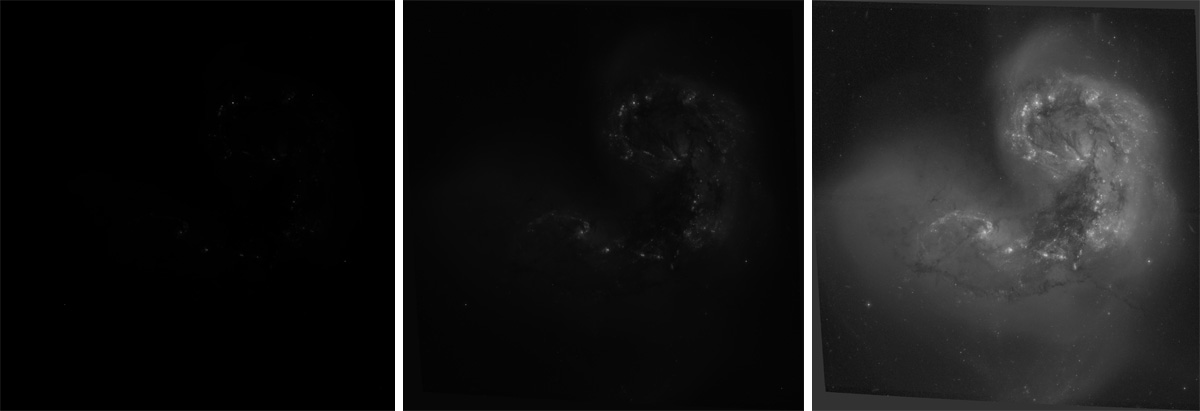
\includegraphics[width=1\textwidth]{images/ecu_lineal_sqr_asinh.jpg}
		\caption{\label{fig:distintasEqu}{\small De izquierda a derecha, imagen ecualizada linealmente, aplicando raíz cuadrada y aplicando arco seno hiperbólico.}}
	\end{figure}
	Se calculan los valores del histograma (ver figura \ref{fig:histLines}) que definen los umbrales con los que se generan tres matrices o imágenes, que denominaremos imagen {\scriptsize Espacio vacío}, imagen {\scriptsize Halo} e imagen {\scriptsize Candidatos}.\\ 
	\begin{figure}[!htb]
		\centering
		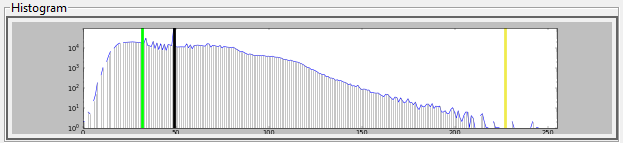
\includegraphics[width=1\textwidth]{images/histLines.png}
		\caption{\label{fig:histLines}{\small Lineas de ecualización sobre histograma.}}
	\end{figure}
	\\
	Estas imágenes o matrices  (ver figura \ref{fig:imagenesAutoGeneradas}), serán usadas en el paso de clasificación.
	\begin{figure}[!htb]
		\centering
		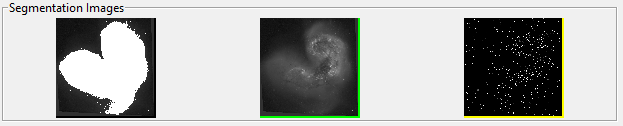
\includegraphics[width=1\textwidth]{images/imagenesAutoGeneradas.png}
		\caption{\label{fig:imagenesAutoGeneradas}{\small Imágenes o matrices autogeneradas que se usarán para la catalogación.}}
	\end{figure}
	\\
	\newpage
	\paragraph{Algoritmo de clasificación}
	Partiendo de una imagen adaptada por el pre-procesado base, se realizan los siguientes pasos que se detallan en el esquema.(Ver figura \ref{fig:esquemaClasificaciosn})\\
	\begin{figure}[!htb]
		\centering
		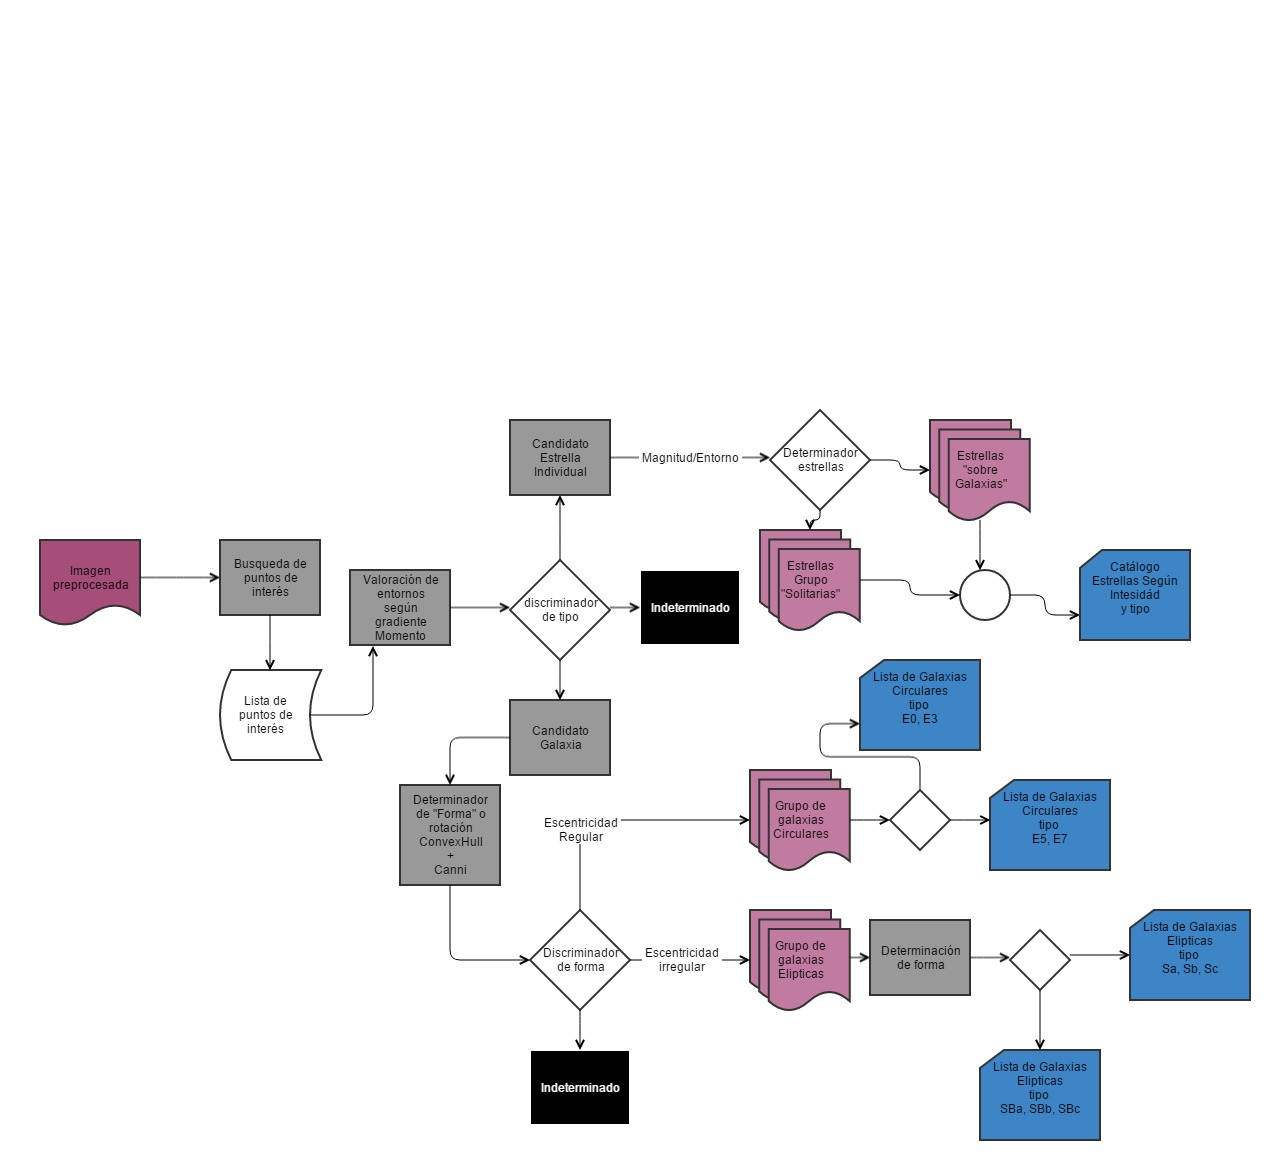
\includegraphics[width=1\textwidth]{images/tfg2016algoritmos_de_catalogaci_n.jpg}
		\caption{\label{fig:esquemaClasificaciosn}Flujo de clasificación}
	\end{figure}
	\\
	\textbf{Obtención de coordenadas de puntos de interés:} \\
	Se genera una lista de candidatos partiendo de la imagen {\scriptsize Candidatos} obtenida tras el pre-procesado.
	
	Para cada coordenada candidata se valorará, mediante su entorno (contenido en la imagen {\scriptsize Halo}), si es un posible candidato a estrella o galaxia. Ciertos puntos se descartarán por ser información espuria (probablemente formados artificialmente en el detector).
	%unificar fig 17 y 18
	Como resultado obtendremos una imagen en la que viene marcados los puntos catalogados como estrellas y las galaxias resaltadas por su contorno (ver figura \ref{fig:estrellasContornos})
	\begin{figure}[!htb]
		\centering
		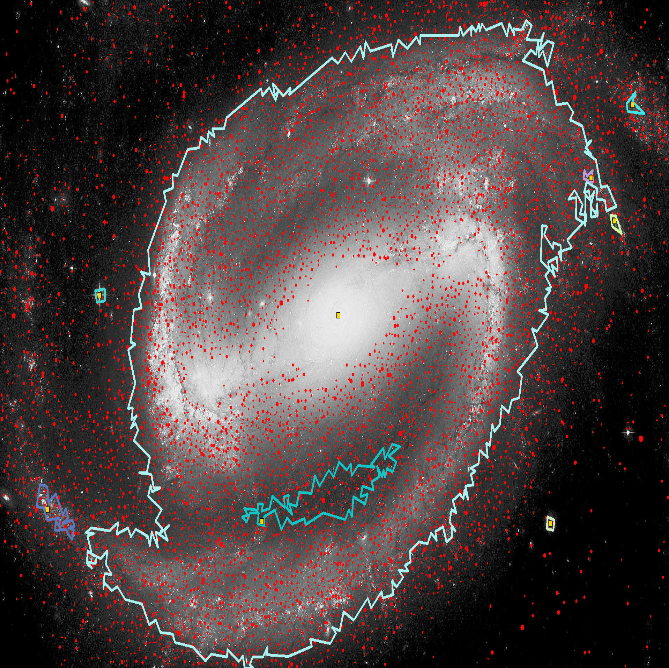
\includegraphics[width=1\textwidth]{images/vectorClasifica.png}
		\caption{\label{fig:estrellasContornos}{\small Resultado de la clasificación. Marcado en rojo parecen las estrellas, los contornos denotan las galaxias.}}
	\end{figure}
	\\
	\textbf{Clasificación de estrellas:}
	\\Para la clasificación de estrellas se usa una aproximación múltiple, primero la detección en base a un umbral (todo conjunto de puntos que tienen intensidad superior a ese umbral pasan a ser candidatos) y segundo la búsqueda de blobs usando OpenCV.\\
	Con los datos generados de ambas aproximaciones se hace un último filtrado que elimina el posible ruido catalogado como candidato. Para ello se hace uso de la imagen-matriz de zonas oscuras, eliminando los puntos que recaen en zonas catalogadas como espacio vacío o ruido.
	\\
	\textbf{Clasificación de galaxias:}\\
	Para la clasificación de galaxias se hace un uso intensivo de búsqueda de contornos, que una vez obtenidos, en base al área media y a su número, se realiza un proceso de eliminación de contornos que no representan galaxias. La parte encargada de la eliminación hace uso de herramientas estadísticas sencillas en nuestro caso hacemos uso de la media de las áreas de los contornos, este valor actúa como umbral, descartándose las áreas inferiores a la mitad del área media, este valor se ha obtenido en base a prueba y error sobre la batería de imágenes.

	\subsection{Interfaz gráfica}\label{GUI}
	Tanto para el usuario final como para la validación de los algoritmos en tiempo real se ha creado una interfaz (Ver figura \ref{fig:GUI_limpia}) que permite: visualización de la imagen, ajuste de una serie de parámetros y presentación visual de los elementos astronómicos detectados.\\
	\begin{figure}[!htb]
		\centering
		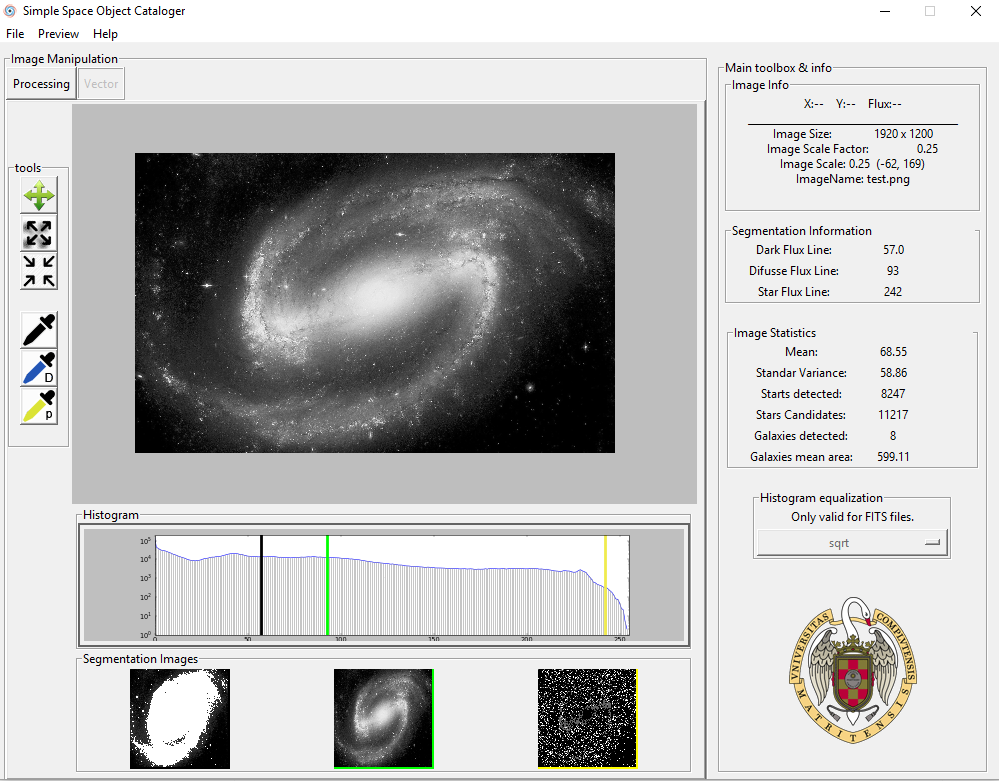
\includegraphics[width=1\textwidth]{images/gui/general.png}
		\caption{\label{fig:GUI_limpia}Interfáz gráfica}
	\end{figure}

	La interfaz gráfica se compone de los siguientes elementos
	\begin{itemize}
		\item Menú superior:
		\newline
		\\Tiene por secciones File, Preview y Help.
			\\File: las opciones que se permiten son la carga de imágenes, el guardado del proyecto y la conversión y guardado (si procede) de una imagen FITS (ver figuras  \ref{fig:menuFile} y \ref{fig:menuFileActive}).
			\begin{figure}[!htb]
				\centering
				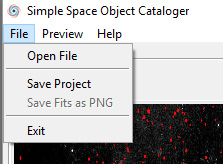
\includegraphics[width=0.3\textwidth]{images/gui/menuFileGhost.jpg}
				\caption{\label{fig:menuFile}{\small Menu Superior con una imagen raster cargada, la opción Save Fits as PNG aparece desactivada.}}
			\end{figure}
			\begin{figure}[!htb]
				\centering
				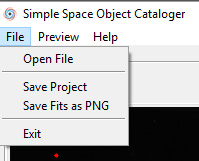
\includegraphics[width=0.3\textwidth]{images/gui/menuFileUnGhost.jpg}
				\caption{\label{fig:menuFileActive}{\small Si cargamos una imagen FITS se activa la opción de convertir y guardar en formato PNG.}}
			\end{figure}
			\newline
			\\Preview: Contiene la opción Invert Image, que invierte la imagen mostrada, esta opción es útil para apreciar mejor (en algunos casos) las diferencias de color (ver \ref{fig:menuPreview}).
			\begin{figure}[!htb]
				\centering
				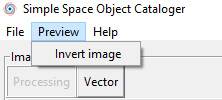
\includegraphics[width=0.3\textwidth]{images/gui/menuPreview.jpg}
				\caption{\label{fig:menuPreview}}
			\end{figure}
			\newline
			\\Help: Sólo contiene una sección About en la que se informa de la versión del software y dónde descargarlo (ver figura \ref{fig:menHelp}).
			\begin{figure}[!htb]
				\centering
				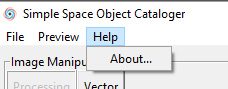
\includegraphics[width=0.3\textwidth]{images/gui/menuHelp.jpg}
				\caption{\label{fig:menHelp}}
			\end{figure}
		\item Zona central:
		\\Muestra el área central de procesado y tiene dos sub-secciones: la sección processing y la sección vector.\\
		La sección Processing es el área principal de trabajo, se muestra la imagen astronómica en tratamiento, el histograma  y las sub-imágenes generadas (ver imagen \ref{fig:histSegImg}) en base a la imagen cargada.\\
					\begin{figure}[!htb]
						\centering
						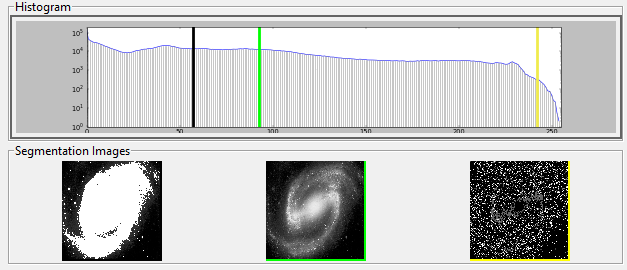
\includegraphics[width=0.7\textwidth]{images/gui/Histogram_segmentation.png}
						\caption{\label{fig:histSegImg}{\small Histograma e imágenes segmentadas}}
					\end{figure}
		\\Contiene también herramientas de navegación (mover, aumentar y reducir la imagen), así como selectores de intensidad para modificar la segmentación de las imágenes (ver imagen \ref{fig:tools}).
					\begin{figure}[!htb]
						\centering
						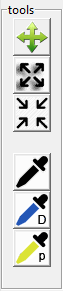
\includegraphics[width=0.05\textwidth]{images/gui/tools.png}
						\caption{\label{fig:tools}{\small Herramientas de navegación y selectores de segmentación}}
					\end{figure}
		Cada pipeta se corresponde con una línea de color del histograma, siendo la primera pipeta en color negro, la que se encarga de manejar la línea de intensidad del espacio vacío, la pipeta de color verde la que maneja la línea de intensidad del halo y la pipeta amarilla la encargada de manejar la línea de intensidad pico relacionada con las estrellas.
		\\
		Al pulsar sobre cualquiera de las pipetas, el cursor cambiará, permitiendo sobre la imagen de trabajo pulsar en cualquier punto para modificar los valores del procesado.
		\newline
		\\
		La sección Vector es el resultado del proceso, en ella se muestra sobre la imagen cargada y procesada, las estrellas y zonas de galaxias encontradas (ver figura \ref{fig:vector}).
			\begin{figure}[!htb]
				\centering
				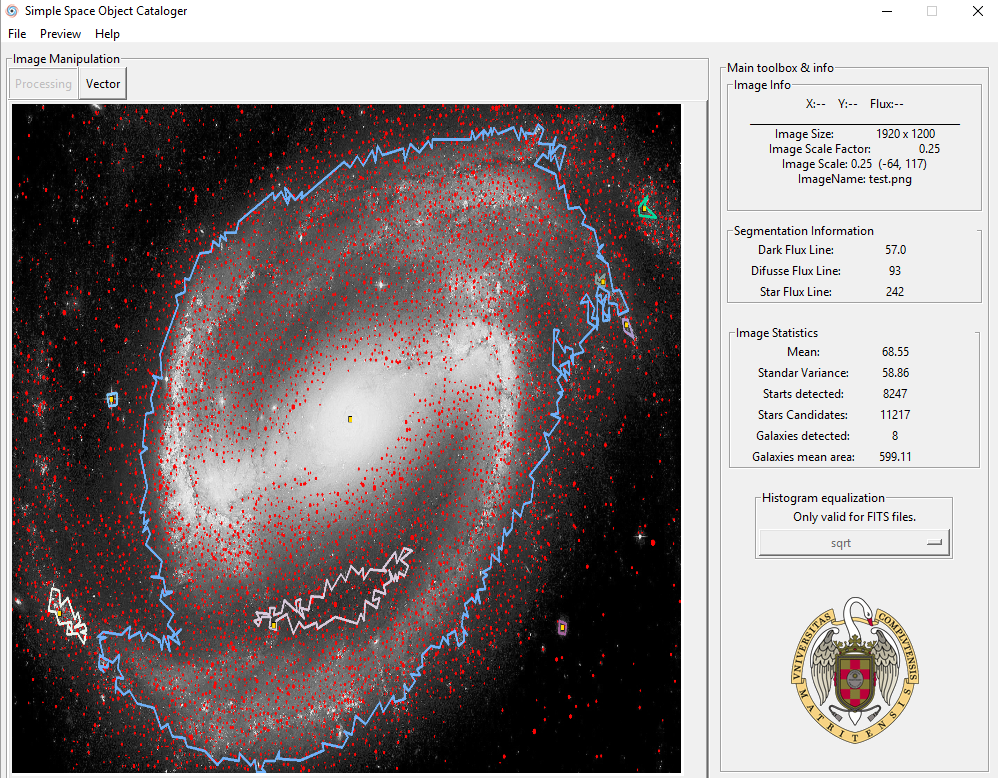
\includegraphics[width=0.7\textwidth]{images/gui/Vector.png}
				\caption{\label{fig:vector}{\small Sección Vector: Resultado del procesado y catalogación.}}
			\end{figure}
		\item Elementos de información y control de equalización (ver figura \ref{fig:BarraDerecha}):
		En la parte derecha de la ventana está presente el cuadro de información que contiene datos estadísticos de la imagen tales como su media y varianza, el número de estrellas o galaxias detectadas y la información del pixel sobre el que tenemos el puntero del ratón.
		\\
			\begin{figure}[!htb]
				\centering
				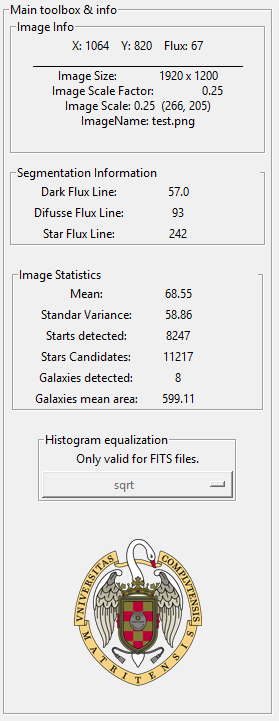
\includegraphics[width=0.2\textwidth]{images/gui/rightBar.png}
				\caption{\label{fig:BarraDerecha}}
			\end{figure}
		En la sección inferior está el selector de ecualización, que nos permite ver cómo se transforma la imagen en función de la ecualización que apliquemos. Esta opción está unicamente disponible cuando el fichero fuente es FITS.
		
	\end{itemize}

	%Conclusiones#########################################################
	\newpage
	\section{Conclusiones}
	%
	Se han desarrollado una serie de funciones y métodos para, dada una imagen con contenido astronómico, detectar elementos astronómicos tales como estrellas y galaxias, todo ello se ha acompañado de una interfaz gráfica que permite visualizar y modificar la ecualización de la imagen para obtener los elementos astronómicos buscados.
	%MODIFICAR
	El desarrollo de este trabajo ha resultado ser un medio de aprendizaje y
	adquisición de nuevos conocimientos teóricos relativos a la astronomía, tales como la existencia de los ficheros FITS, la compresión de su contenido, la clasificación de galaxias según la secuencia de Hubble ( o diagrama diapasón), necesarios para el desarrollo de este trabajo.
	El uso de OpenCV ha hecho que adquiera conocimientos en el área de visión artificial, concretamente destaco la detección de contornos.
	El hecho de desarrollar un proyecto con interfaz gráfica, ha provocado que adquiera conocimientos en el área de usabilidad y programación de librerías gráficas, en este caso concreto con Tkinter.
	También ha sido una búsqueda de soluciones a los errores y problemas que se presentaban, principalmente en la ecualización de las imágenes FITS en los que se ha hecho uso de conocimientos matemáticos en las transformaciones de dominio.\\ \\

	%MODIFICAR
	Se ha conseguido, llegar a un prototipo de software, abierto a realizar nuevas mejoras tal como se detallará en la sección \ref{sec:futureWork}, aplicando técnicas conocidas durante el desarrollo de este trabajo, pero que no ha sido posible incorporar tales como la substracción de cielo.
	%FIN MODIFICAR
	\\
	\newline

	\subsection{Cumplimiento de objetivos}
	El resultado del proyecto es un software funcional, rápido y manejable que cumple con los objetivos básicos planteados y en el que se deja la puerta abierta a mejoras y nuevas funcionalidades que quedaron descartadas debido a la complejidad que presentaban en función del tiempo con el que contaba.
	\\Cada una de las metas propuestas inicialmente cumple su cometido.\\
	Los problemas que se han presentado durante la realización han sido:\\
	\begin{itemize}
		\item Durante el desarrollo se han tenido que descartar propiedades tales como la clasificación detallada de la morfología de las galaxias, la complejidad es superior a la estimada incialmente, y para obtener un prototipo con las máximas funcionalidades, se han pospuesto.
		\item Las peculiaridades de la imagen astronómica hacen difícil estimar ciertas características. Un ejemplo claro es el siguiente:\\
			Las imágenes fuente pueden incluir, en el caso de pertenecer a alguna misión astronómica, zonas sobre-expuestas, esto es debido a que el aparato de captación fue configurado para obtener datos de un punto poco luminoso, haciendo que el resultado sea una imagen que contiene sobre-exposición en zonas más luminosa. Este es uno de los muchos inconvenientes con los que el software se encuentra a la hora de calibrar la imagen y obtener las lineas de intensidad sobre, datos con los que se realiza todo el proceso.
	\end{itemize}
	\subsection{Trabajo futuro}
	\label{sec:futureWork}
	Tal y como se ha comentado anteriormente, se ha dejado una puerta abierta a mejoras:
	\begin{itemize} 
	\item Para la detección de espacio vacío o \textit{sky substraction} se ha echo uso de un estimador basado en la media de intesidad de la imagen, para un mejor funcionamiento sería necesario analizar el artículo \cite{BlantonSubstraction}, concretamente el apartado \textit{2.2. Masking the data} y adaptarlo a nuestro procesamiento de imágenes.
	\item Los ajustes estadísticos, realizados en base a un pequeño conjunto de imágenes, requieren afinamiento, no se descarta tomar nuevas estrategias \cite{SSDImgPro}, por ejemplo en la obtención de los contornos de los candidatos a galaxias establecer una relación entre el área y el perímetro para de este modo detectar estructuras que presenten crestas o pliegues (ver en figura \ref{fig:MembraneNebulae}, página \pageref{fig:MembraneNebulae})
		\begin{figure}[!htb]
			\centering
			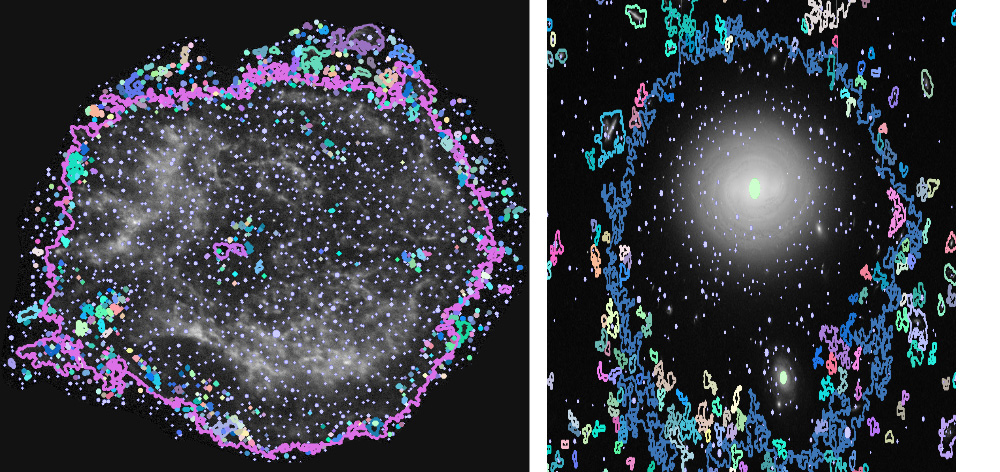
\includegraphics[width=0.7\textwidth]{images/nebulaMembrana2.jpg}
			\caption{\label{fig:MembraneNebulae}{\small El comportamiento de los contornos presenta excesivos pliegues en la imagen de la derecha (tono azul) en comparación con el comportamiento de la imagen de la izquierda (tono violeta).El contorno de la derecha es un claro ejemplo de contorno erróneo.}}
		\end{figure}
	\item Mejoras de optimización. Un claro ejemplo es la detección de estrellas y galaxias que se pueden unificar en una única función, o la gestión de las imágenes internas que en algunos (thumbnails) casos se duplican innecesariamente ocupando temporalmente memoria.
	\item Añadir la funcionalidad de clasificación acorde a la secuencia de Hubble (ver figura \ref{fig:EsquemaHubble}), para ello, todo el proceso previo ha de ser óptimo en sus resultados y se ha de contar con sistema de categorización de contornos ellipticos.
				\begin{figure}[!htb]
					\centering
					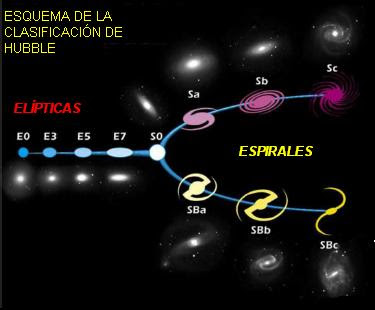
\includegraphics[width=0.5\textwidth]{images/EsquemaHubble.jpg}
					\caption{\label{fig:EsquemaHubble}{\small Secuencia del doctor Hubble para la clasificación de galaxias.}}
				\end{figure}
	\item Otro punto interesante podría ser la creación de un método que detecte los destellos de lente o lens flare (ver figura \ref{fig:lensflare}), ya que nuestro algoritmo los puede interpretar como galaxias, por su halo en determinados casos.
			\begin{figure}[!htb]
				\centering
				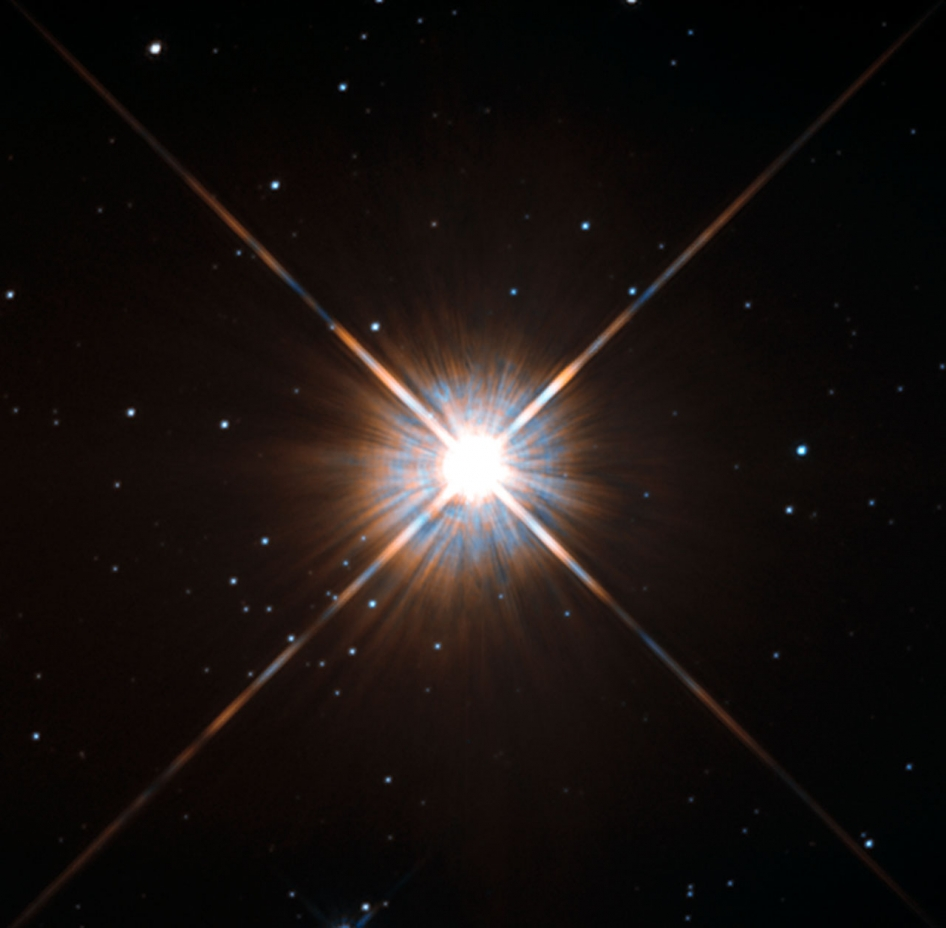
\includegraphics[width=0.2\textwidth]{images/HubbleProximaCentauri_LENSFLARE}
				\caption{\label{fig:lensflare}Lens flare en una captura producida pro el telescopio Hubble de Proxima Centaury. Imagen cortesía de  ESA/Hubble NASA.}
			\end{figure}
	\end{itemize} 

	%Agradecimientos#######################################################
	\newpage
	\section{Agradecimientos}
	
	Quiero agradecer a Carlos Gregorio Rodríguez la oportunidad de realizar este trabajo fin de grado, la ayuda y guía que me ha brindado en todo momento y su apoyo en la búsqueda de soluciones y la adquisición de nuevos conocimientos.\\ 
	\\ A Miguel Angel Valero Espada por darme un enfoque distinto de lo que es el campo de la programación. Ana Inés Gomez de Castro y a Fátima López Martínez por sus enseñanzas en Astronomía.\\
	\\ Muy especialmente a Rocío por animarme en todo momento y estar siempre a mi lado, así como a mi familia por su apoyo.\\
	\\ Sin todos ellos me hubiese resultado muy difícil el desarrollo del proyecto.
	\\
	\\Éste trabajo está dedicado especialmente a mi yeyos Mercedes y Modesto por todos los valores que desde bien pequeño me supieron transmitir.
	\newpage
%Referencias bibiográficas#############################################
	%\section{Referencias bibiográficas}
	%Se han usado tanto Pappers académicos de distintos ámbitos, publicaciones y documentación %de las librerías usadas.\\

	\begin{thebibliography}{1}
		\bibitem{NASADISKHALO}\textsc{Barnes, Joshua E.} \\
		\textit{Encounters of disk/halo galaxies}
		\textit{Astrophysical Journal, Part 1 (ISSN 0004-637X), vol. 331, Aug. 15, 1988, p. 699-717.}
		\\1988
		\\http://articles.adsabs.harvard.edu//full/1988ApJ...331..699B/0000699.000.html
		
  		\bibitem{OpenCV}\textsc{Willow Garage et all.} \\
  		\textit{OpenCV: Open Source Computer Vision. Documentación oficial.}
  		\\http://docs.opencv.org/
		\\Intel's research center in Nizhny Novgorod
  		\\2.000 (v:1.0) - 2015 (v:3.0)

  		\bibitem{PajaresCruzUCM}\textsc{Gonzalo Pajares, Jesús M. de la Cruz} \\
  		\textit{Visión por computador: Imágenes digitales y aplicaciones}
  		\\ISBM: 84-7897-472-5.
  		\\2.001 RA-MA Editorial.

	  	\bibitem{SSDImgPro}\textsc{Robert Lupton.} \\
	  	\textit{SDSS Image Processing I: The Deblender.}
	  	\\http://www.astro.princeton.edu/~rhl/photomisc/deblender.pdf
		\\2.001 Princeton University Observatory
	  
  		\bibitem{NasaFITS}\textsc{NASA/GSFC} \\
  		\textit{The FITS Support Office - Documentación oficial formato FITS.}
  		\\http://fits.gsfc.nasa.gov/
	  	
	  		  	
		%Referenciada
	  	\bibitem{stellarOutcast}\textsc{ David A. Aguilar, Christine PulliamPublic } \\
	  	\textit{First Stellar Outcast Discovered by Astronomers}
	  	\\https://www.cfa.harvard.edu/news/2005-05
	  	\\2.005 Harvard-Smithsonian Center for Astrophysics
	  
  	  	\bibitem{BlantonSubstraction}\textsc{Michael R. Blanton et all.} \\
  	  	\textit{Improved background subtraction for the Sloan Digital Sky Survey images.}
  	  	\\http://arxiv.org/pdf/1105.1960.pdf 
  	  	\\2.011
	\end{thebibliography}
\end{document}